% !TEX TS-program = xelatex
% !BIB program = biber
% !TEX encoding = UTF-8 Unicode

% 使用手冊請見 TW_Thesis_Template wiki:
% https://github.com/sppmg/TW_Thesis_Template/wiki

% User guide in wiki of TW_Thesis_Template :
% https://github.com/sppmg/TW_Thesis_Template/wiki

\documentclass[openany]{NTHU_thesis} % \documentclass[option1, option2, ...]
% Helpful options: 
% draft = Don't load figure ,reduce compile time.
% showframe = show document margins.
% colorgrid = show colored coordinate. (by eso-pic pkg.)
% openany: see issue #5, NTHU not allow blank page, so add this option to allow chapter start in left side,
\usepackage[subpreambles]{standalone} % standalone class setting in config.tex
% Option ``subpreambles'' enable sub-tex's preambles when compile main tex. (pkg default disable)
% sppmg think it's still some problem (e.g. \addbibresource will faild ), recommend move all subpreambles to ``macros_preamble.tex``
\usepackage{mathrsfs,amsmath}


\begin{document}
    \frontmatter
        % \documentclass[class=NTHU_thesis, crop=false, float=true]{standalone}
\begin{document}
% I use LaTeX3 to automatically generate name table. 
% Below \ExplSyntaxOn to \ExplSyntaxOff perpare prof. table contents,
% it will save contents to `\profsTableContent''. 
% You can ignore this block even you want make table by yourself.
\ExplSyntaxOn
% Copy prof. list from config.tex
\clist_gclear_new:N \g_sppmg_profsZh_cl
\clist_gset:NV \g_sppmg_profsZh_cl \profsZh
\clist_gclear_new:N \g_sppmg_profsEn_cl
\clist_gset:NV \g_sppmg_profsEn_cl \profsEn

% get total number of prof. . Omitted language will not display.
\int_gzero_new:N \g_sppmg_profTotal_int
\int_gset:Nn \g_sppmg_profTotal_int {
    \int_max:nn {\clist_count:N \g_sppmg_profsZh_cl} 
        {\clist_count:N \g_sppmg_profsEn_cl}
}

% NOTE: ``tabularx'' will  processes its contents more than once 
% for calculate width, so ``gpop'' can't put in tabularx env.
% \tl_if_exist:NTF {\tl_clear:N \g_sppmg_tableContent_tl} {\tl_new:N \g_sppmg_tableContent_tl}
% \tl_if_exist:NTF \g_sppmg_tableContent_tl {} {\tl_new:N \g_sppmg_tableContent_tl}
\tl_gclear_new:N \g_sppmg_tableContent_tl


% Use a inline function for pop 2 list (zh+en), and save table content 
% Input(#1) switch 3 case, 1 = Advisor, 2 = committee member , 3+ is more.
% Use ``for'' loop to get all prof.
\int_step_inline:nnnn {1}{1}{\g_sppmg_profTotal_int}{
    \clist_gpop:NNTF \g_sppmg_profsZh_cl \l_tmpa_tl {}{ \tl_clear:N \l_tmpa_tl}
    \clist_gpop:NNTF \g_sppmg_profsEn_cl \l_tmpb_tl {}{ \tl_clear:N \l_tmpb_tl}
    \tl_gput_right:Nx \g_sppmg_tableContent_tl {
        \int_case:nnTF {#1}{
            {1} {指導教授: & \l_tmpa_tl & 博士 & (Dr.~ \l_tmpb_tl ) \exp_not:n {\\} }
        }{}{
            & \l_tmpa_tl & 教授 & (Prof.~ \l_tmpb_tl ) \exp_not:n {\\} 
        }
    }
}

% Copy contents to LaTeX2e macro.
\cs_set_eq:NN \profsTableContent \g_sppmg_tableContent_tl

\ExplSyntaxOff
\def\fsUniversity{\fs{24}[1.5]}
\def\fsTitle{\fs{20}[1.5]}
\def\fsNames{\fs{18}[1.5]}

\def\mcShift{\hspace{-6.0pt}} % It's for align non-multicolumn cell .
% --------define title page layout for thesis
\titlepageFontFamily % set in config.tex
\newgeometry{top=2.5cm, bottom=2.5cm, inner=2cm, outer=2cm} % only for titlepage
\begin{spacing}{1.0}
\begin{titlepage}
    \null\vfill
    \begin{center}
        {\fsUniversity 國\quad 立\quad 清\quad 華\quad 大\quad 學} \par
        \vspace*{5mm}
        
        {\fsTitle {\degree}論文\par}
        \vspace*{20mm}
        
        {\fsTitle {\title} \par}
        \vspace*{5mm}
        
        {\fsTitle {\subtitle} \par}
        \vspace*{10mm}
        
        {\ifx \logo\empty\vspace*{30mm}
        \else \includegraphics[height=30mm]{\logo} \par
        \fi}
        \vfill
        
        {\fsNames \renewcommand{\arraystretch}{1}
            % If you want make table by yourself, replace ``\profsTableContent''
            \begin{tabular}{l@{\hspace*{0.4em}}l@{\quad}l@{\quad}l}
            系\qquad 所: & \multicolumn{3}{l}{\mcShift \dept}      \\
            學\qquad 號: & \multicolumn{3}{l}{\mcShift \studentID} \\
            研\enspace 究\enspace 生: & \authorZh & & (\authorEn)    \\
            
            \profsTableContent
            
            \end{tabular}
        \par}
        \vspace*{5ex}
        
        {\fsTitle {\degreedate} \par}
        \vspace*{2ex}
        
        \ifthenelse{\boolean{printcopyright}}
        {{{版權所有\copyright\ \author\ \quad \copyyear} \par}}
        {}
    \end{center}
    \null\vfill
\end{titlepage}
\end{spacing}
\restoregeometry
\normalfont % use main font
%--------end of title page for thesis
\cleardoublepage
\end{document}
       % 封面(不加浮水印)
        \documentclass[class=NTHU_thesis, crop=false, float=true]{standalone}
\begin{document}
% I use LaTeX3 to automatically generate name table. 
% Below \ExplSyntaxOn to \ExplSyntaxOff perpare prof. table contents,
% it will save contents to `\profsTableContent''. 
% You can ignore this block even you want make table by yourself.
\ExplSyntaxOn
% Copy prof. list from config.tex
\clist_gclear_new:N \g_sppmg_profsZh_cl
\clist_gset:NV \g_sppmg_profsZh_cl \profsZh
\clist_gclear_new:N \g_sppmg_profsEn_cl
\clist_gset:NV \g_sppmg_profsEn_cl \profsEn

% get total number of prof. . Omitted language will not display.
\int_gzero_new:N \g_sppmg_profTotal_int
\int_gset:Nn \g_sppmg_profTotal_int {
    \int_max:nn {\clist_count:N \g_sppmg_profsZh_cl} 
        {\clist_count:N \g_sppmg_profsEn_cl}
}

% NOTE: ``tabularx'' will  processes its contents more than once 
% for calculate width, so ``gpop'' can't put in tabularx env.
% \tl_if_exist:NTF {\tl_clear:N \g_sppmg_tableContent_tl} {\tl_new:N \g_sppmg_tableContent_tl}
% \tl_if_exist:NTF \g_sppmg_tableContent_tl {} {\tl_new:N \g_sppmg_tableContent_tl}
\tl_gclear_new:N \g_sppmg_tableContent_tl


% Use a inline function for pop 2 list (zh+en), and save table content 
% Input(#1) switch 3 case, 1 = Advisor, 2 = committee member , 3+ is more.
% Use ``for'' loop to get all prof.
\int_step_inline:nnnn {1}{1}{\g_sppmg_profTotal_int}{
    \clist_gpop:NNTF \g_sppmg_profsZh_cl \l_tmpa_tl {}{ \tl_clear:N \l_tmpa_tl}
    \clist_gpop:NNTF \g_sppmg_profsEn_cl \l_tmpb_tl {}{ \tl_clear:N \l_tmpb_tl}
    \tl_gput_right:Nx \g_sppmg_tableContent_tl {
        \int_case:nnTF {#1}{
            {1} {指導教授: & \l_tmpa_tl & 博士 & (Dr.~ \l_tmpb_tl ) \exp_not:n {\\} }
        }{}{
            & \l_tmpa_tl & 教授 & (Prof.~ \l_tmpb_tl ) \exp_not:n {\\} 
        }
    }
}

% Copy contents to LaTeX2e macro.
\cs_set_eq:NN \profsTableContent \g_sppmg_tableContent_tl

\ExplSyntaxOff
\def\fsUniversity{\fs{24}[1.5]}
\def\fsTitle{\fs{20}[1.5]}
\def\fsNames{\fs{18}[1.5]}

\def\mcShift{\hspace{-6.0pt}} % It's for align non-multicolumn cell .
% --------define title page layout for thesis
\titlepageFontFamily % set in config.tex
\newgeometry{top=2.5cm, bottom=2.5cm, inner=2cm, outer=2cm} % only for titlepage
\begin{spacing}{1.0}
\begin{titlepage}
    \null\vfill
    \begin{center}
        {\fsUniversity 國\quad 立\quad 清\quad 華\quad 大\quad 學} \par
        \vspace*{5mm}
        
        {\fsTitle {\degree}論文\par}
        \vspace*{20mm}
        
        {\fsTitle {\title} \par}
        \vspace*{5mm}
        
        {\fsTitle {\subtitle} \par}
        \vspace*{10mm}
        
        {\ifx \logo\empty\vspace*{30mm}
        \else \includegraphics[height=30mm]{\logo} \par
        \fi}
        \vfill
        
        {\fsNames \renewcommand{\arraystretch}{1}
            % If you want make table by yourself, replace ``\profsTableContent''
            \begin{tabular}{l@{\hspace*{0.4em}}l@{\quad}l@{\quad}l}
            系\qquad 所: & \multicolumn{3}{l}{\mcShift \dept}      \\
            學\qquad 號: & \multicolumn{3}{l}{\mcShift \studentID} \\
            研\enspace 究\enspace 生: & \authorZh & & (\authorEn)    \\
            
            \profsTableContent
            
            \end{tabular}
        \par}
        \vspace*{5ex}
        
        {\fsTitle {\degreedate} \par}
        \vspace*{2ex}
        
        \ifthenelse{\boolean{printcopyright}}
        {{{版權所有\copyright\ \author\ \quad \copyyear} \par}}
        {}
    \end{center}
    \null\vfill
\end{titlepage}
\end{spacing}
\restoregeometry
\normalfont % use main font
%--------end of title page for thesis
\cleardoublepage
\end{document}
       % 書名頁
        % \listoftodos   % todo list, hide when set \textbackslash{}setboolean\{publish\}\{\textbf{true}\} in config.tex. It will not add to TOC , you can add \todototoc before \listoftodos to do that.

        %%%%%%%%%%%% letters %%%%%%%%%%%%
        % Set file name in config.tex
        % 依校方規定,此處須插入:
        % [v] 清大(電子授權書) 必備,不論是否授權都要裝訂
        % [v] 清大(紙本授權書) 必備,不論是否授權都要裝訂
        % [x] 國家圖書館(電子授權書) 有授權才要裝訂
        % [v] 國家圖書館(紙本論文延後公開/下架申請書)→紙本論文有申請延後公開才要裝訂
        % [v] 指導教授推薦書
        % [v] 考試委員審定書
        % !!! [x] 部份請自行插入

        % 碩博士論文電子檔授權書 Authorization Letter (for electronic)
        \IfFileExists{\letterAuthEl}{
            \cleardoublepage        % 由下個右頁開始
            \includepdf{\letterAuthEl}}{}
        % 碩博士論文紙本授權書 Authorization Letter (for paper)
        \IfFileExists{\letterAuthPa}{
            \cleardoublepage        % 由下個右頁開始
            \includepdf{\letterAuthPa}}{}
        % 國家圖書館(電子授權書) 有授權才要裝訂

        % 碩博士紙本論文延後公開/下架申請書。(如需延後公開者,才需要裝訂於論文內頁)
        \IfFileExists{\letterPubReq}{
            \cleardoublepage
            \includepdf{\letterPubReq}}{}
        % 指導教授推薦書
        \IfFileExists{\letterRecom}{
            \cleardoublepage
            \includepdf{\letterRecom}}{}
        % 口試委員審定書
        \IfFileExists{\letterVerif}{
            \cleardoublepage
            \includepdf{\letterVerif}}{}
        \cleardoublepage
        
        %%%%%%%%%%%% Other frontmatter, eg,abstract %%%%%%%%%%%%
        % 中英文論文摘要:內容應說明研究目的,資料來源,研究方法及研究結果等
        \documentclass[class=NCU_thesis, crop=false]{standalone}
\begin{document}

\chapter{摘要}
在此寫上你的中文摘要。

\vspace{2em}
\noindent \textbf{關鍵字:} \keywordsZh{} % Set keywords in config.tex
\end{document} % zh 中文摘要
        \documentclass[class=NCU_thesis, crop=false]{standalone}
\begin{document}

\chapter{Abstract}
In classical communication, spread spectrum technology is an effective way to improve the security in transmission process. We try to implement this technology in quantum communication as well. In our experiment, we have used synchronized high-speed electro- optic modulators to modulate the phase of resonant single photon and biphoton wave packets, which are generated from cavity enhanced SPDC (spontaneous parametric down-conversion) and broaden their bandwidths from 4.5 MHz to 10 GHz for avoiding photons being absorbed or detected by the atoms. The reduced absorption is like imposing an invisible cloak over a photon, improving the confidentiality during the transmission process in order to improve the security of quantum communication and key distribution. 

In principle, atoms will absorb on-resonant narrowband (smaller than natural linewidth) single photons in our experiment. we broadened the bandwidth of the photon to a wide range between 2~10 GHz, with the absorption rate decreasing to 70~30\% By these results, our work shows that, for transmitted photons, the higher the bandwidth, the higher the confidentiality.

\vspace{2em}
% \noindent \textbf{Keywords:} \keywordsEn{} % Set keywords in config.tex
\end{document} % en 英文摘要
        \documentclass[class=NCU_thesis, crop=false]{standalone}
\begin{document}

\chapter{誌謝}

謝謝天謝謝地

\end{document}


 % 誌謝(可略)

        % 原始 book class 不將 TOC,LOF,LOT 加入目錄列表,須手動加
        % 此樣板可由 config.tex 切換是否自動加入目錄
        \tableofcontents        % 目錄
        \listoffigures          % 圖目錄
        \listoftables           % 表目錄
        % \documentclass[class=NCU_thesis, crop=false]{standalone}
\begin{document}

\chapter{使用符號與定義}
這裡示範用表格做符號與定義列表。你也可以利用套件``nomencl''(簡易)或``glossaries''(強大)完成,詳細說明見教學(v1.8+)。

\begin{table}[h]
    \normalsize % 使用與內文一樣大的字體,請自調
    \centering
    \begin{tabular}{c@{\quad:}l}
%         符號     & 說明 \\ 
        VIM     & 用vim的是神 \\ 
        Emacs   & 神在用的編輯器 \\ 
        CTAN    & Comprehensive TeX Archive Network, ctan.org \\
        
    \end{tabular} 
    \caption*{符號與定義} % 不想顯示請註解/刪除\caption行(\label自動失效)
    \label{table:symbol_def}
\end{table}

\end{document}
    % 符號說明
    \mainmatter
        \documentclass[class=NCU_thesis, crop=false]{standalone}
\begin{document}

\chapter{實驗背景與動機}
\section{古典通訊展頻}
展頻技術 (Spread Spectrum Technology) \cite{simon1985spread,pickholtz1982theory}在古典通訊上已行之有年,最初為軍事或情報單位傳遞資訊使用,以避免電波干擾或訊號攔截,現今此技術以廣泛運用無線電通訊中。

根據 FCC(Federal Communications Committee;美國聯邦通訊委員會)規定的 ISM(Industrial, Scientific and Medical)頻帶,在特定頻段內不需申請執照即可供民間、工業、科學與醫學用途使用,由於任何設備可自由使用這些頻段來傳遞訊息,這些頻段上會十分擁擠,訊號可能會互相影響,如\cref{fig:jamming},而使用展頻技術即可解決此頻段共享的問題。一般而言展頻技術主要可分成跳頻展頻(Frequency Hopping Spread Spectrum, FHSS)和直接序列展頻(Direct Sequence Spread Spectrum, DSSS),以下簡單介紹這兩者的原理與應用。


\fig[0.5][fig:jamming][!htb]{jamming.png}[同頻訊號干擾。綠色發送端發出之訊號,紅色為其他訊號源發出之同頻訊號干擾。][同頻訊號干擾]

藍芽技術上,使用的頻段為 2.4 GHz,在 ISM 規範的波段內,會與無線電話、無線網路等設備共享頻段,若同時有兩個以上訊號使用同樣的頻率來傳輸,由於接收端無法區分訊號的來源,會相互干擾,想克服此問題可使用跳頻技術:傳輸端每秒改變訊號的頻率數次,接收端以對應的頻率去接收訊號,示意\cref{fig:fhss},如此可避免特定頻段遭占用的問題。

\begin{figure}[!hbt]
    %\captionsetup[subfigure]{labelformat=empty} % 完全隱藏圖號
    \centering
    \subcaptionbox
        {Channel assignment
        \label{fig:fhss_channel_assignment}}
        {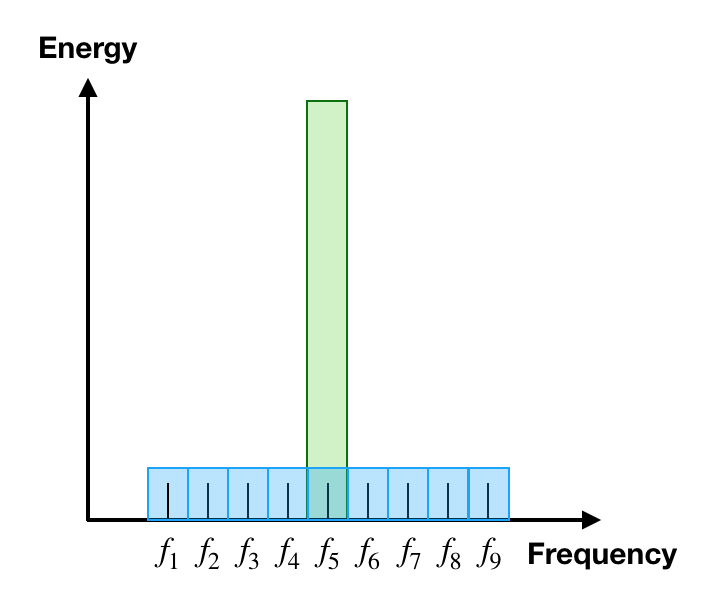
\includegraphics[width=0.4\linewidth]{fhss_channel_assignment.png}}
    ~~~~
    \subcaptionbox
        {Chaneel use
        \label{fig:fhss_channel_use}}
        {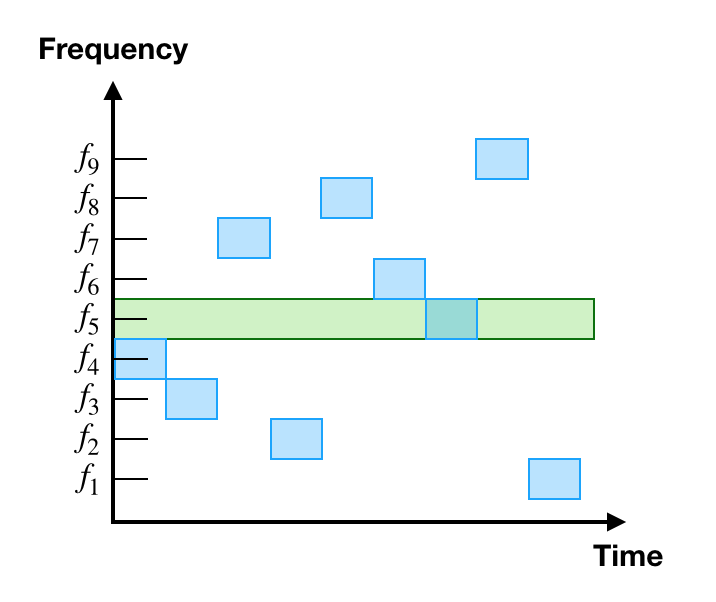
\includegraphics[width=0.4\linewidth]{fhss_channel_use.png}}
    \caption[跳頻展頻技術示意圖]{跳頻展頻技術示意圖,綠色為展頻前,藍色為展頻後。\cref{fig:fhss_channel_assignment} 為指定的頻率分佈,展頻前僅使用 $f_5$ 這個頻率通道進行傳輸,展頻後則將訊號分成數個頻率,不同時間以不同頻率進行傳輸,如\cref{fig:fhss_channel_use}}
    \label{fig:fhss}
\end{figure}

直接序列展頻技術則是以一串特定的高頻訊號,對發動端的原始資訊進行調製,時域上的調製過程如\cref{fig:dsss_process}。

\fig[1][fig:dsss_process][!htb]{dsss_process.png}[直接序列展頻技術調製過程。綠色為發送端要傳輸之原始資訊;紅色為高頻偽隨機訊號,用來對綠色訊號進行相位調製,調製的結果為藍色訊號。接收端可使用紅色訊號對藍色訊號進行解碼,即可還原出原始的綠色訊號][直接序列展頻技術調製過程]

上述的調製過程能將頻譜展寬,如\cref{fig:dsss_spread},接收端會再以相同的高頻訊號對其進行解碼,還原出原始的資訊。此種方式可以有效的降低同頻訊號的干擾,示意圖如\cref{fig:dsss}。DSSS 提供一種穩定且簡單的解決方案,能以低功率高頻寬遠距傳輸資訊,廣泛應用於無線網路、無線電話、GPRS...等,但相較於跳頻展頻技術,直接序列展頻技術需要較高的硬體建置成本。

\fig[0.5][fig:dsss_spread][!htb]{dsss_spread.png}[直接序列展頻技術,對原始訊號進行調製且展寬其頻寬。綠色為調製前的窄頻資訊,藍色為調製後的展頻資訊,其頻寬與調製的速度成正比,用越高速的訊號進行調製能使頻寬展至越寬][直接序列展頻技術,對原始訊號進行調製,增加訊號之頻寬。]

\begin{figure}[!hbt]
    %\captionsetup[subfigure]{labelformat=empty} % 完全隱藏圖號
    \centering
    \subcaptionbox
        {展頻後傳輸之訊號
        \label{fig:dsss_spread_jamming}}
        {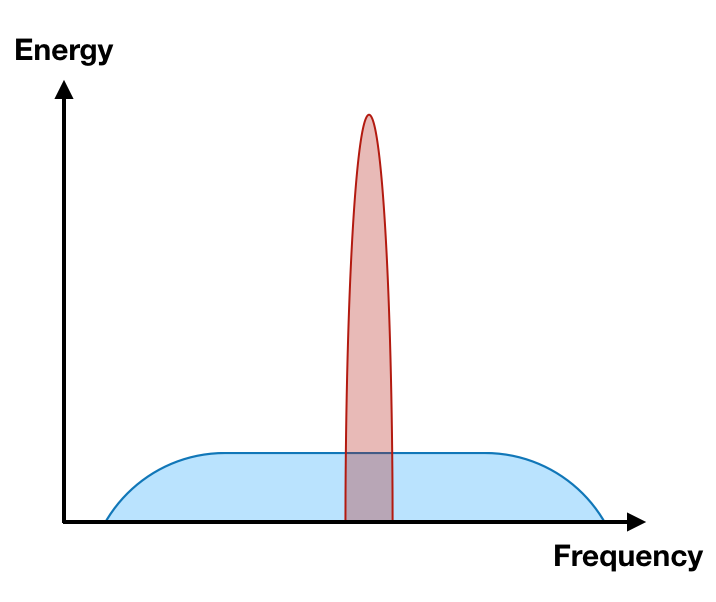
\includegraphics[width=0.4\linewidth]{dsss_spread_jamming.png}}
    ~~~~
    \subcaptionbox
        {解展頻後之接收訊號
        \label{fig:dsss_compress_jamming}}
        {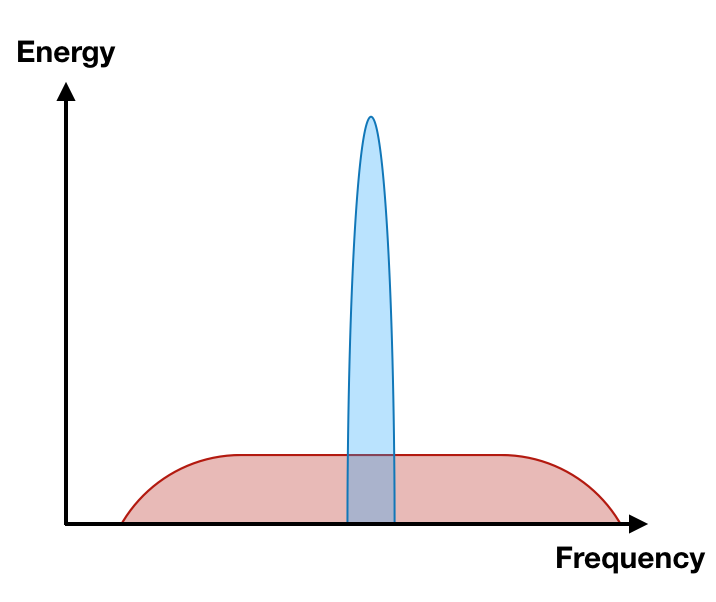
\includegraphics[width=0.4\linewidth]{dsss_compress_jamming.png}}
    \caption[直接序列展頻技術示意圖]{直接序列展頻技術示意圖。\cref{fig:dsss_spread_jamming} 藍色為已展頻之發送端訊號,紅色為同頻訊號干擾。\cref{fig:dsss_compress_jamming} 為接收端解展頻後的訊號,藍色訊號被回復成原始的狀態,紅色的同頻訊號則被展頻,能量被打散至各個不同的頻率,可降低接收端的收到的雜訊。}
    \label{fig:dsss}
\end{figure}

\section{量子通訊展頻}
在量子資訊中,有許多的應用是以單光子作為攜帶資訊的媒介,展頻後的光能以低功率高頻寬的狀態被傳輸,甚至還能將資訊藏於雜訊中\cite{belthangady2010hiding},此外,以量子密鑰分發\cite{RevModPhys.74.145}而言,DPS-QKD (differential phase shift quantum key distribution)\cite{PhysRevLett.89.037902} 提供了傳輸密鑰的方式,但卻無法確保訊號能在不被干擾的情況下抵達接收端,所以若能將展頻技術應用在單光子上,降低環境或人為干擾對遠距傳輸的影響,則可提升資料傳輸的效率與安全性。

此外,若想將單光子的量子態儲存於磁光陷阱中的 $^{87}Rb$ 冷原子作為量子記憶體使用\cite{PhysRevLett.101.120501},由於  $^{87}Rb$ 原子的自然線寬約為 6 MHz,此方法能大幅度降低光子對對於 $^{87}Rb$ 的吸收率,避免資訊遭第三方惡意竊取。

\section{研究簡介}
基於上述之實驗背景與動機,我們研究的目的為將展頻技術運用於單光子上,在第二章中會介紹展頻的原理,從數學的角度去探究相位調製對頻譜的影響;第三章中會以前一章的數學原理,以我們的實驗的條件進行模擬,並計算當光子與原子產生交互作用下時的頻譜變化;第四章介紹實驗上會用到的重要儀器;第五章介紹實驗的流程並討論實驗結果,最後再針對實際測量到的結果對理論進行修正與比較。

\end{document}    % 緒論
        \documentclass[class=NCU_thesis, crop=false]{standalone}
\usepackage{mathrsfs,amsmath}
\begin{document}


\end{document}          % 基本原理介紹
        \documentclass[class=NCU_thesis, crop=false]{standalone}
\usepackage{mathrsfs,amsmath}

\begin{document}

\chapter{理論模擬}
\section{展頻及壓縮}
從上一章單頻波的例子可看出,相位調製可將原先頻率集中於 $\nu_{0}$ 的光,分散至 $\nu_{0}\pm\nu_{m}, \nu_{0}\pm2\nu_{m},\dots$。若調製函數改用時間寬度為 $\Delta T$ 的隨機方波 $PRBS(t)$ (如\cref{fig:PRBS_simulation}),則可將\cref{eq:modulation_function} 的右式寫成:
\begin{equation}
    \tilde{E_{0}}(\omega)*\mathscr{F}\{{e^{i PRBS(t)}}\}
\end{equation}
經計算,展寬後的頻譜如\cref{fig:spread_sprectrum_simulation},其包絡線接近 $sinc$ 的平方,展開的寬度為 $\pm\frac{1}{\Delta T}$,在我們實驗中使用的隨機訊號的產生率為 10 Gb/s,單一位元的時間寬度為 100 ps,相當於能將頻譜從數 MHz 展至 10 GHz 寬。

\fig[0.5][fig:PRBS_simulation][!htb]{prbs.png}[隨機訊號 $PRBS(t)$]

\fig[0.5][fig:spread_sprectrum_simulation][!htb]{temp.png}[展寬後頻譜模擬圖]

經展頻後的訊號,在傳輸的過程中可以降低環境的影響,避免光子被特定原子團吸收,但若想還原光子初始相位的資訊,則需要做一個反向的相位調製,讓光子再經過第二台 EOM,輸入的電訊號必須為與 $PRBS(t)$ 互補的 $\overline{PRBS}(t)$,這兩個訊號要滿足以下關係:

\begin{equation}
    \label{eq:prbs_condition}
    PRBS(t)+\overline{PRBS}(t)=0
\end{equation}
或

\begin{equation}
    e^{i PRBS(t)}\times e^{i \overline{PRBS}(t)}=1
\end{equation}

若光子在兩台 EOM 行經的時間間距為 $\Delta t_{p}$,兩個電訊號抵達的時間差為 $\Delta t_{RF}$,當 $\Delta t_{p}=\Delta t_{RF}$ 時,理論上可以對相位進行反向的調製,將展頻後的訊號壓縮,還原成原本的頻率分布,但若 $\Delta t_{p}>\Delta t_{RF}$,則無法完全還原頻譜,比較如\cref{fig:electric_mismatch},所以在實驗架設上,必須要能精確的控制電路與光路的長度,讓兩個電訊號匹配,才能達到最好的還原效果。

\fig[0.5][fig:electric_mismatch][!htb]{temp.png}[$\Delta t_{p}>\Delta t_{RF}$ 時壓縮頻譜]

\todo[inline]{補上壓縮模擬圖,確定要不要有不 match 時的狀況}

\section{$^{87}Rb$ 原子氣體吸收}

\subsection{展頻對吸收率的影響}
\label{section:simulation_absorption}
在光通訊中,以光作為資訊的載體,在空氣中傳輸的過程中光子會與原子產生交互作用,當光子的頻率接近原子的耀遷能階時有很大的機率會被吸收。以波長約為 795  nm 的窄頻雷射為例,將此道光打入溫度約 70 度的 $^{87}Rb$ 原子氣體管,調整入射光頻率測量穿透率即可掃出 $^{87}Rb$ 的吸收譜,結果如\cref{fig:rb87_abs},從圖中可知,在頻率 105 GHz 與 112 GHz 的頻率位置分別約有 2GHz 與 1 GHz 寬的吸收區域,其吸收的中心頻率是被原子的能階給決定,可從飽和吸收光譜 (saturated absorption spectroscopy) 得知;吸收的寬度則是與原子蒸氣壓和溫度有關,不同的原子運動速度分佈會有不一樣的寬度,此為效應都卜勒增寬 (Doppler broadening)。

\fig[0.75][fig:rb87_abs][!htb]{absorption_spectrum.png}[$^{87}Rb$ 原子吸收譜]

為降低環境對光子的影響,我們可用上述之展頻技術,對光進行相位調製,將頻譜展寬,減少光對原子的吸收率。我們分別使用 1 Gb/s、5 Gb/s、10 Gb/s 與 20 Gb/s 的隨機訊號去模擬,在有展頻的狀態下,中心頻率與穿透率之關係,結果如\cref{fig:different_gbs_transmission},未經調製的光在 105 GHz 與 112 GHz 附近會被完全吸收,若將光的頻譜展寬則能顯著的降低吸收率,隨機訊號的頻率越高,原子對光子的影響越小。

\fig[0.75][fig:different_gbs_transmission][!htb]{different_gbs_spectroscopy.png}[展頻頻寬對吸收之影響。使用越快的隨機訊號對光進行相位調製,能降低光在原子躍遷能階附近的吸收率。][展頻頻寬對吸收之影響]

\subsection{吸收對頻譜還原的影響}
如前所述,對已調製過的光進行反向的調製,理論上可將頻譜壓窄,完美還原成調製前的頻率分佈。但若先讓已展頻的光通過原子團使其被部分吸收,再進行反向的調製,則還原回來的頻譜會與原先有些微的差異,比較如\cref{fig:compress_comparison}。

\fig[0.5][fig:compress_comparison][!htb]{temp.png}[展頻後吸收對壓縮之影響]

\todo[inline]{補上被部分吸收後的壓縮的模擬圖}

\end{document}      % 理論模擬
        \documentclass[class=NCU_thesis, crop=false]{standalone}
\begin{document}

\chapter{實驗儀器與優化流程}

\section{隨機訊號產生器}
由於實驗上無法產生真正的隨機訊號,只能使用偽隨機訊號產生器 (Pseudo Random Bit Sequence, PRBS),儀器型號為 Anritsu 的 MP1763C,可以產生 0.5 至 12.5 Gb/s 的訊號。偽隨機訊號實際上為週期訊號,會重複出現特定的隨機序列,其週期可以調整,為了達到最接近隨機的效果,我們選擇使用最長的隨機序列,一個週期內共有 $2^{31}-1$ 的隨機位元。

我們實驗上實際使用的頻率為 10 GHz (或 10 Gb/s),每秒能產生 $10\times 10^{9}$ 個隨機位元,以示波器去測量該訊號的眼圖 (eye diagram) 則可以知道訊號的品質,量測結果如\cref{fig:prbs_eye},可見實際訊號與理論\cref{fig:PRBS_simulation} 有很大的差異,實際的訊號有著相對大的上升與下降時間,圖形上下也不太對稱,這都會影響到展頻與壓縮的效果,造成實驗與理論的誤差。

\begin{figure}[!hbt]
    %\captionsetup[subfigure]{labelformat=empty} % 完全隱藏圖號
    \centering
    \subcaptionbox
        {第一台 EOM
        \label{fig:subfig_fig1}}
        {\includegraphics[width=0.4\linewidth]{data.bmp}}
    ~~~~
    \subcaptionbox
        {第二台 EOM
        \label{fig:subfig_fig2}}
        {\includegraphics[width=0.4\linewidth]{data_bar.bmp}}
    \caption{PRBS 輸出之訊號眼圖(放大前)}
    \label{fig:prbs_eye}
\end{figure}

\section{電光調製器}
電光調製器 (Electro-Optic Modulator, EOM) 可使用電訊號對光進行調製,一般而言可以分成三種,分別為振幅、相位與偏振的調製,在我們的實驗中需要調製的是相位。使用的儀器為 EOSPACE 的 SN73717 與 SN73718,分別為頻譜的窄寬與壓縮用。

相位調制器由鈮酸鋰 ($LiNbO_{3}$) 雙折射晶體製成,因泡克耳斯效應 (Pockels effect),外加電場能線性的改變快軸上的折射率,進而達到改變相位的效果,且我們稱能將 45 度線偏旋轉至 -45 度的電壓為 $V_{\pi}$。

由上介紹可知,實際使用上需優化進光的偏振以及電訊號的振幅,以達到預期的相位調製效果。

我們使用半波片 (half-wave plate) 調整入射 EOM 偏振的方向,若偏振方向不對的話,調製效果會不佳,如圖\cref{fig:imperfect_polarization},所以實驗上優化的方式為,看著調製後的頻譜,將偏振旋轉到最接近理論模擬時的角度。

\begin{figure}[!hbt]
    %\captionsetup[subfigure]{labelformat=empty} % 完全隱藏圖號
    \centering
    \subcaptionbox
        {入射光為線偏且剛好對準晶體快軸
        \label{fig:perfect_polarization}}
        {
\includegraphics[width=0.4\linewidth]{temp.png}}
    ~~~~
    \subcaptionbox
        {入射光為線偏但沒對準晶體快軸
        \label{fig:imperfect_polarization}}
        {
\includegraphics[width=0.4\linewidth]{temp.png}}
    \caption{入射 EOM 光的偏振對相位調製之影響}
    \label{fig:prbs_eye}
\end{figure}

\section{高頻電訊號放大器}
由於我們使用的隨機訊號產生器僅能輸出 0.2 至 2 $V_{pp}$ 的訊號,EOM 的 $V_{\pi}$ 高於 2 V,需再經過放大器才能提供足夠的電壓去進行相位調製。
同樣的,也用示波器去測量眼圖,看放大後的訊號品質,如\cref{fig:amp_prbs_eye}

\begin{figure}[!hbt]
    %\captionsetup[subfigure]{labelformat=empty} % 完全隱藏圖號
    \centering
    \subcaptionbox
        {第一台 EOM
        \label{fig:subfig_fig1}}
        {\includegraphics[width=0.4\linewidth]{amp_data.bmp}}
    ~~~~
    \subcaptionbox
        {第二台 EOM
        \label{fig:subfig_fig2}}
        {\includegraphics[width=0.4\linewidth]{amp_data_bar.bmp}}
    \caption{PRBS 輸出之訊號眼圖(放大後)}
    \label{fig:amp_prbs_eye}
\end{figure}

由於兩台放大器連接 EOM 使用的 SMA 線的材質與長短不同,會有不一樣的頻率響應與耗損,使兩個訊號無法互補,這會對頻譜壓縮與還原的效果造成負面的影響。

\section{法布立-培若干涉儀}
古典光可以用法布立-培若 (Fabry-Perot) 干涉儀來掃出頻譜,我們使用的儀器為 THORLABS 的(型號),FSR 為 10 GHz。
此干涉儀的主體為一個共振腔,由兩面高反射率的鏡子所組成。當光垂直入射腔體時,須滿足以下共振條件的光才能會有建設性干涉,能透射共振腔:

\begin{equation}
    2nL=m\lambda
\end{equation}
n 為共振腔的折射率,L 為腔長,頻率與透射率做圖,其中 $\nu_{F}$ 稱為 FSR (Free Spectrual Range),此參數決定了這個干涉儀適用的掃頻範圍,調整腔長 L 的大小能改變允許透射的頻率,所以若在其中一面鏡子黏上 Piezo ,輸入電壓即可微調腔長,達到掃頻的效果。

\fig[0.5][fig:label][!htb]{temp.png}[Fabry-Perot 干涉儀透射頻率]
此外,另一個重要的參數為 F (Finesse),為精細度,定義如下:

\begin{equation}
    F=\frac{\pi R^{1/2}}{1-R}
\end{equation}
此共振腔的頻寬(解析度) $\delta \lambda$ 與 F 成反比,關係如下式,所以鏡面反射率越高,F越大,解析度越好,此次實驗使用的干涉儀解析度約為 60 MHz。

\begin{equation}
    \delta \lambda=\frac{\nu_{F}}{F}
\end{equation}

\section{Etalon 干涉儀}
與 Fabry-Perot 干涉儀為相同的原理,但 Fabry-Perot 干涉儀的共振腔體為自由空間 (free space),而 Etalon 干涉儀的共振腔體則為一塊雙折射晶體,我們可以用 TEC 和溫控器,精準的調控晶體溫度 T 改變腔長 $L(T)$,只讓特定中心頻率 $\nu$ 附近的光通過。我們實驗使用的型號為 AF023G (MICRO OPTICS, INC.),頻寬為 60 HMz,FSR 為 13.6 GHz。

由於腔體是由雙折射晶體製成,所以不同的偏振在內部會有不一樣的行進速度,而會產生兩組不同的模態,所以在實驗優化上,需要將入射 Etalon 干涉儀的光調成符合
其中一個晶軸的線偏光,才能最有效率的使用這濾波器。

\end{document}          % 實驗方法與架設
        \documentclass[class=NCU_thesis, crop=false]{standalone}

\begin{document}
\chapter{實驗架設與結果討論}
本章為實驗的主軸,會從光源的製備出發,說明實驗上會用到兩種不同光源的產生機制。再介紹光路的架設與其測量上限制,且會在同樣的架設下,分別以兩種不同的光源去測量,交叉驗證不同系統下實驗的結果,並與前幾章的理論計算比較,探討可能產生誤差的原因,以實際的狀況去修正理論模擬,讓計算結果更貼近測量數據,

\section{光源製備}

\subsection{雷射光}
雷射光源為 TOPTICA 的 DLC TA-SHG PRO 雷射系統,可產生中心波長約為 795 nm 的窄頻雷射。此雷射的特點為出光頻率可調,可以透過電壓控制共振腔上光柵的角度來調整出光的頻率。

除了波長 795 nm 的紅外,雷射系統內還有一塊在共振腔內的非線性晶體,可將前述的紅光打入內,產生倍頻效應 (SHG) 產生波長為 397.5 nm 的藍光,可用來打入另一塊非線性晶體,以自發參量下轉換 (Spontaneous Parametric Down-Conversion, SPDC) 的過程產生 975 nm 的光子。


\subsection{單光子}
\label{subsection:single_photon}
雙光子的產生機制為 SPDC,入射一道波長 397.5 nm 的藍光雷射進入 PPKTP 晶體,產生 Type-II 的時間 - 能量糾纏光子對 (time-energy entangled biphoton),波長為 795 nm。

藉由在 PPKTP 晶體雙邊鍍上 795nm 的高反射薄膜,右邊鍍上 397.5 nm 的高反射薄膜,可形成一個共振腔,讓產生出來的光子對有相對長的相干時間 (coherence time) 與較窄的頻寬。

實驗上會將產生出來的雙光子對經過 PBS,將訊號分為 signal 和 idler,以 idler 做為觸發訊號,使 signal 經過 $^{87}Rb$ 原子氣體管與 EOM,讓光子被吸收或對其進行相位的調製,並做 $G^{2}(\tau)$ 的測量,$G^{2}(\tau)$ 的定義如 (\ref{eq:g2_definition})。

\begin{equation}
    G^{2}(\tau)=\frac{4\Gamma_{s}\Gamma_{i}}{\Gamma_{s}+\Gamma_{i}}\left\{\begin{matrix}
        e^{\Gamma_{s}\tau} & ,\tau<0\\
        e^{-\Gamma_{i}\tau} & ,\tau>0
        \end{matrix}\right.
\label{eq:g2_definition}
\end{equation}

此為二階強度關聯函數 (second-order intenstiy correlation function),$\tau$ 為兩顆單光子抵達探測器的時間差。在符合準相位匹配條件 (quasi phase matching condition) 時能最有效率的產生雙光子,實際測量結果如\cref{fig:single_photon_g2},此光子之時間波包寬度約為 100 ns,頻寬為 4.5 MHz。

\fig[0.75][fig:single_photon_g2][!htb]{nocell_spread_no_etalon.png}[糾纏光子對之 $G^{2}(\tau)$ 量測]


為了找到符合準項未匹配條件的入射光波長與晶體溫度,實驗上我們先將入射光的頻率固定在 105489 MHz,改變晶體溫度測量雙光子的產生率 (biphton rate),結果如\cref{fig:temp_scan_g2}黑線,在 39.91$^{\circ}C$ 至 40.10$^{\circ}C$ 有四組符合條件的模態,若讓其中一顆光子經過 $^{87}Rb$ 原子氣體管,並做相同的量測,結果如\cref{fig:temp_scan_g2}紅線,可以發現第二和第三個的模態雖有明顯的吸收,但吸收率不高,我們認為這是因為晶體所產生的光子為多模 (multi-mode) 而非單模 (single-mode),同時產生了兩種以上頻率的單光子,儘管其中一個頻率的光子能完全被吸收,其他頻率的光子仍會透射,因此無法讓透射率趨近於零。為了確認這想法,我們在探測器前面加上一個頻寬為 60 MHz 的 Etalon 濾波器,只允許特定頻率附近的光通過,並在沒放 $^{87}Rb$ 原子氣體管時改變晶體溫度,重新測量產生率,有無 Etalon 濾波器測量之結果比較如\cref{fig:temp_scan_g2_with_etalon},黑色為沒放 Etalon 濾波器時測量到的訊號,紅色經過濾波後之訊號,兩者相比可明顯看出,有放濾波器時能將其他產生效率較低的模態過濾掉,一次只讓一個特定頻率區間內的光通過。此時再將 $^{87}Rb$ 原子氣體管放回,並對其中第二和第三個模態進行相同的量測,結果如\cref{fig:absorption_etalon_temp_scanning},黑線為加上 Etalon 過濾之後測到的訊號,若放上 $^{87}Rb$ 原子氣體管讓光子通過,測量結果如藍線,光子幾乎完全被吸收,與\cref{fig:temp_scan_g2}相比,可明顯看出,在過濾前的光源的確有其他頻率的成分,要避免其他頻率成分影響後續的實驗與分析,需加上 Etalon 濾波器。

\fig[0.75][fig:temp_scan_g2][!htb]{temp_scanning.png}[調整溫度測量雙光子產生率,黑線為直接對雙光子進行量測;紅線為先讓其中一顆單光子通過 $^{87}Rb$ 氣體管再測量,其中第二和第三個模態有部分吸收。][調整溫度測量雙光子產生率]

\fig[0.75][fig:temp_scan_g2_with_etalon][!htb]{temp_scanning_with_etalon.png}[黑色為無濾波器時測量之訊號,在二與三個模態附近測量到一些明顯的訊號,表示我們的單光子非單模;紅線為經過濾波器測量到的訊號,此時就只允許特定頻率透射。][調整溫度測量雙光子產生率(加上濾波器)]

\begin{figure}[!hbt]
    %\captionsetup[subfigure]{labelformat=empty} % 完全隱藏圖號
    \centering
    \subcaptionbox
        {第二個模態
        \label{fig:subfig_fig1}}
        {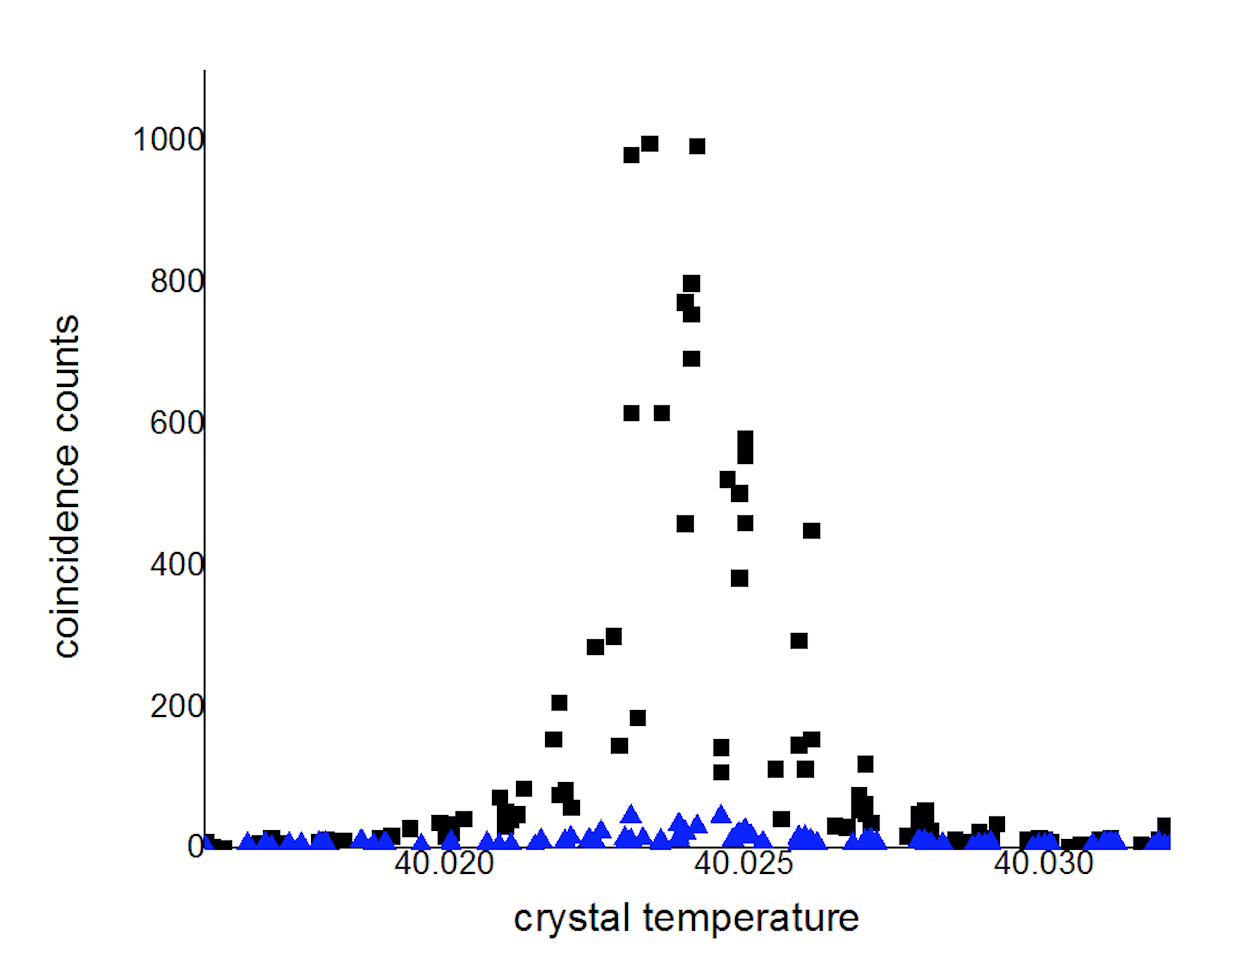
\includegraphics[width=0.4\linewidth]{second_mode_absorption.png}}
    ~~~~
    \subcaptionbox
        {第三個模態
        \label{fig:subfig_fig2}}
        {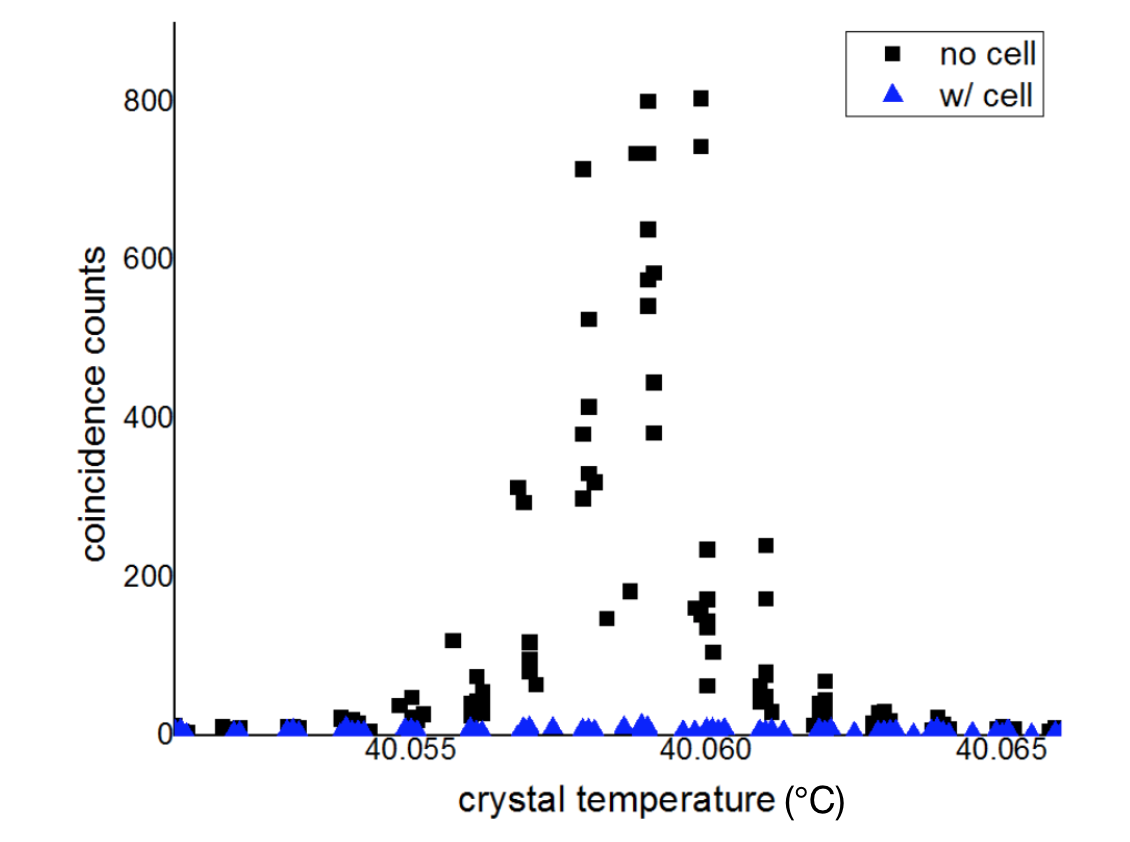
\includegraphics[width=0.4\linewidth]{third_mode_absorption.png}}
    \caption{經過 Etalon 濾波後光子之吸收}
    \label{fig:absorption_etalon_temp_scanning}
\end{figure}

\section{雷射頻譜量測}

實驗光路架設如\cref{fig:laser_spectrum_setup},我們將窄頻雷射通過兩台 EOM 對其進行相位調製,第一台為展頻用,第二台用來做反向的調製還原頻譜,再以 Fabrty-Perot 干涉儀去測量頻譜。

\fig[0.75][fig:laser_spectrum_setup][!htb]{laser_spectrum_setup.png}[雷射頻譜量測光路圖]

在兩台 EOM 都關閉的情況下,可以測到波長 795 nm 雷射的頻譜,結果如\cref{fig:laser_spectrum},以此 Fabry-Perot 的解析度掃出的雷射頻寬約為 60 MHz。

\fig[0.75][fig:laser_spectrum][!htb]{laser_spectrum.png}[以頻寬 60MHz 的 Fabry-Perot 干涉儀掃出之雷射頻譜][雷射頻譜]


若只開啟第一台 EOM,在 10 Gb/s 隨機訊號的調製下可將窄頻雷射光的頻譜展至 10 GHz 寬,但由於我們的使用的 Fabry-Perot FSR 僅 10 GHz,無法涵蓋完整的頻率區間,會使測量的結果失真,要想掃出完整展開的頻譜需使用 FSR 20 GHz 以上的干涉儀,所以下面會先以 2 Gb/s 的訊號來測試展頻的結果是否符合理論模擬。

\subsection{2 Gb/s 隨機訊號之相位調製}
先以 2 Gb/s 隨機訊號進行相位調製,只開啟第一台能將頻譜展至 $\pm$5 GHz 寬,如\cref{fig:2gbs_spread}。

\fig[0.75][fig:2gbs_spread][!htb]{2_31_spread_2GHz.png}[2 Gb/s 訊號之展頻頻譜]

頻譜的形狀大致上與理論相符,但在 $\pm$2 GHz 的位置有一個突起的訊號,這是由於隨機訊號的上升與下降時間不夠快所致,若在數值模擬中把隨機訊號加上約 100 ps 的上升與下降時間(如\cref{fig:simulation_rising_falling_prbs}),則會出現類似的結果,如\cref{fig:simulation_rising_falling}。

\begin{figure}[!hbt]
    %\captionsetup[subfigure]{labelformat=empty} % 完全隱藏圖號
    \centering
    \subcaptionbox
        {修正前隨機訊號
        \label{fig:subfig_fig1}}
        {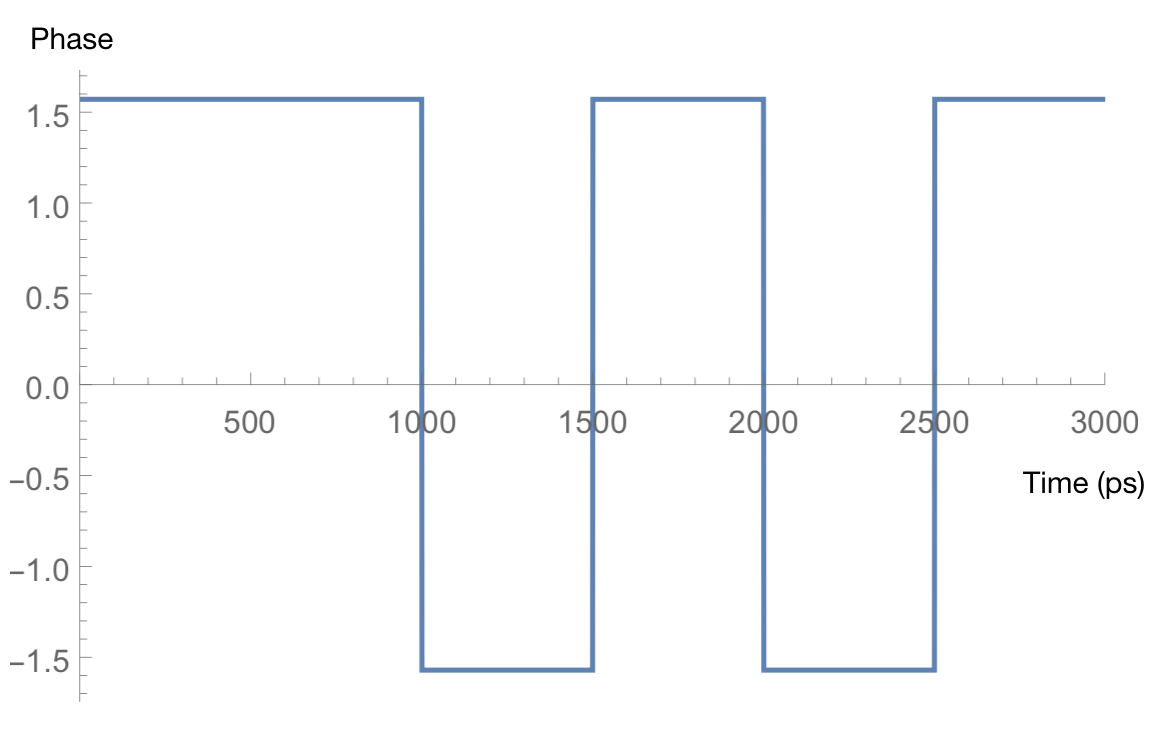
\includegraphics[width=0.4\linewidth]{2gbs_prbs.png}}
    ~~~~
    \subcaptionbox
        {修正後隨機訊號
        \label{fig:subfig_fig2}}
        {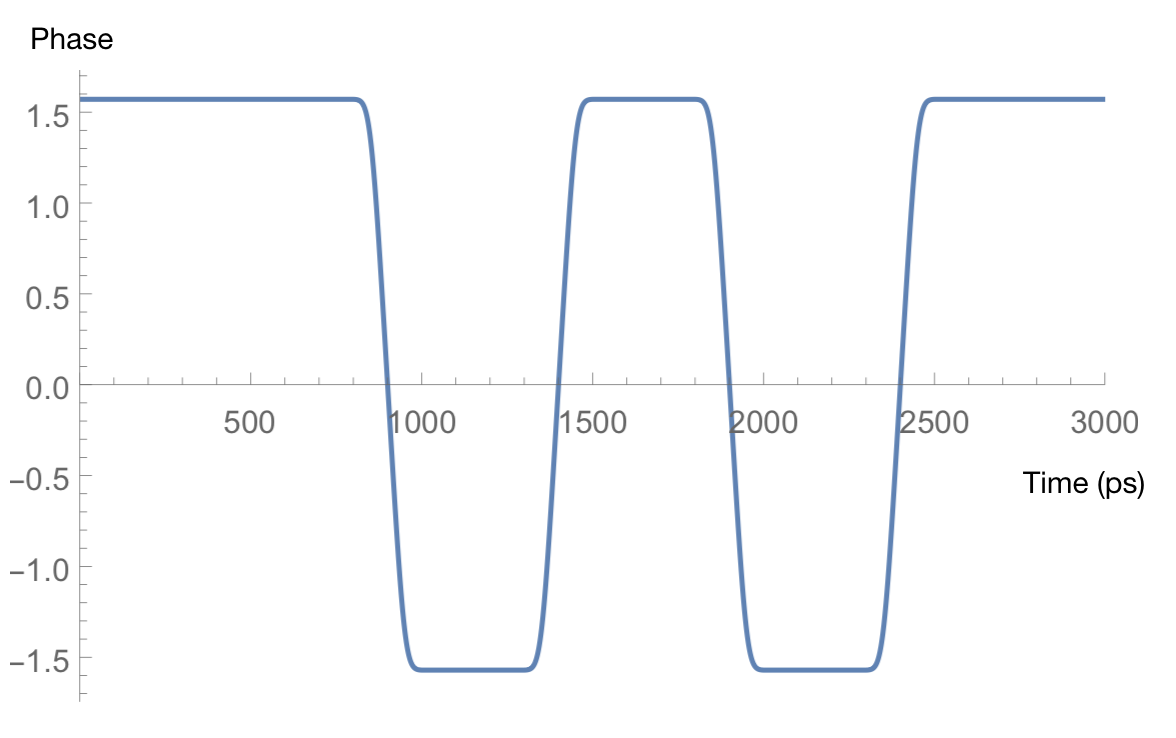
\includegraphics[width=0.4\linewidth]{2gbs_prbs_rf.png}}
    \caption{隨機訊號修正,加上上升時間與下降時間。}
    \label{fig:simulation_rising_falling_prbs}
\end{figure}

\begin{figure}[!hbt]
    %\captionsetup[subfigure]{labelformat=empty} % 完全隱藏圖號
    \centering
    \subcaptionbox
        {修正前展頻模擬
        \label{fig:subfig_fig1}}
        {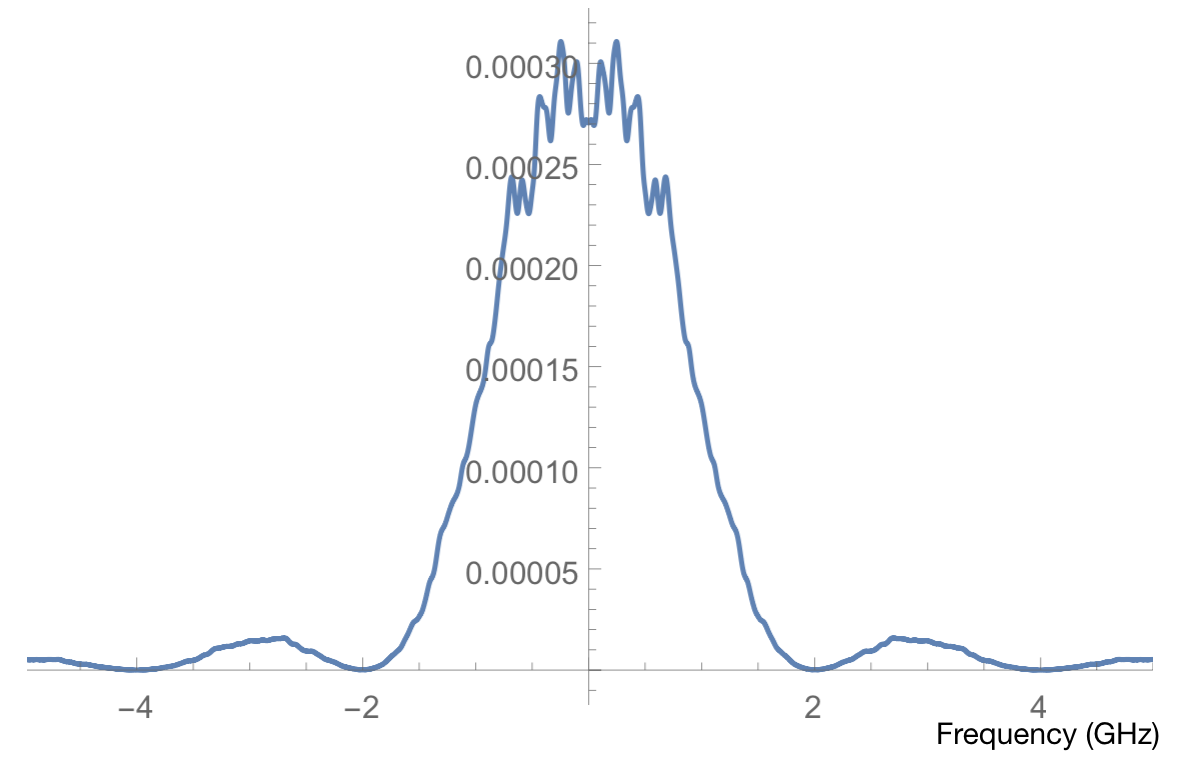
\includegraphics[width=0.4\linewidth]{2gbs_spread.png}}
    ~~~~
    \subcaptionbox
        {修正後展頻模擬
        \label{fig:subfig_fig2}}
        {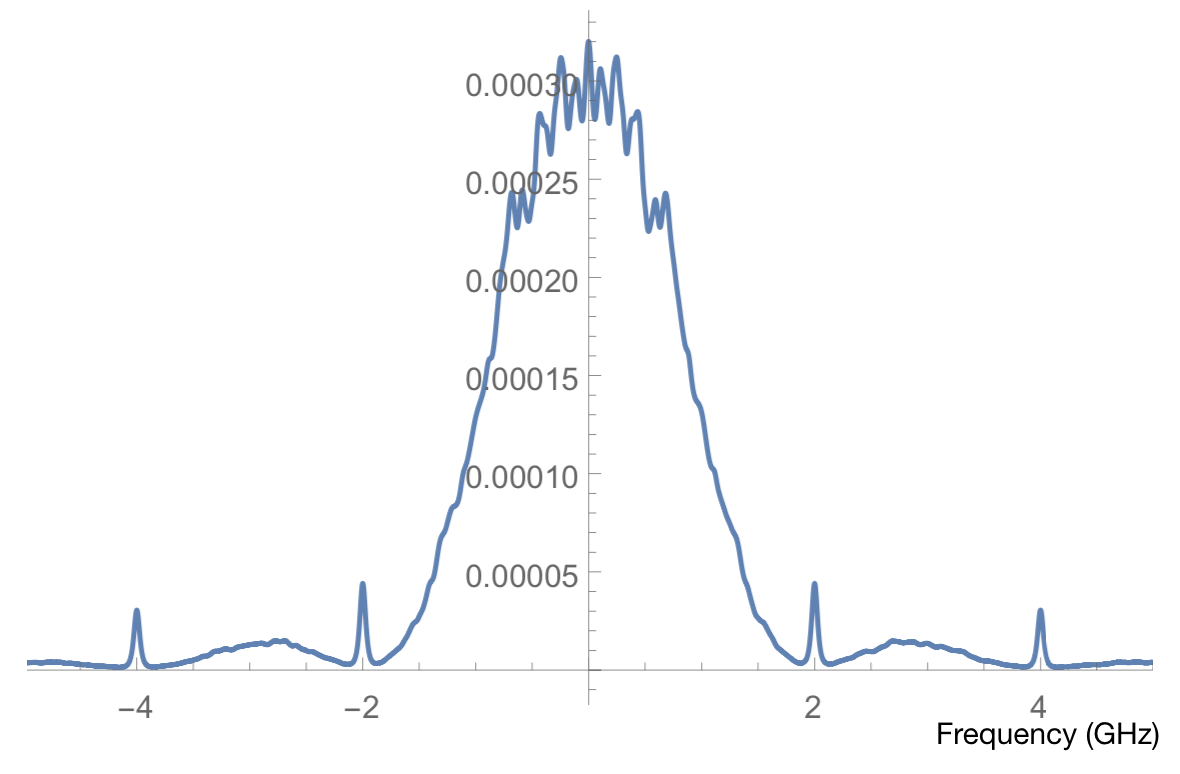
\includegraphics[width=0.4\linewidth]{2gbs_spread_rf.png}}
    \caption{隨機訊號之上升與下降時間對頻譜之影響,隨機訊號加了上升與下降時間後的模擬更貼近實驗結果。}
    \label{fig:simulation_rising_falling}
\end{figure}

\todo[inline]{隨機訊號模擬圖,展頻模擬圖}

此外,還可隱約看出該頻譜的包絡線有週期振盪的訊號,原因為我們使用的隨機訊號實際上是個重複出現的週期訊號,每個週期有 $2^{31}-1$ 個位元,若把位元數調為 $2^{15}-1$ 或者 $2^{7}-1$ 則可看到週期更大的震盪訊號,測量結果如\cref{fig:different_length_PRBS}。

\begin{figure}[!hbt]
    %\captionsetup[subfigure]{labelformat=empty} % 完全隱藏圖號
    \centering
    \subcaptionbox
        {週期 $2^{15}-1$ 位元之偽隨機訊號
        \label{fig:subfig_fig1}}
        {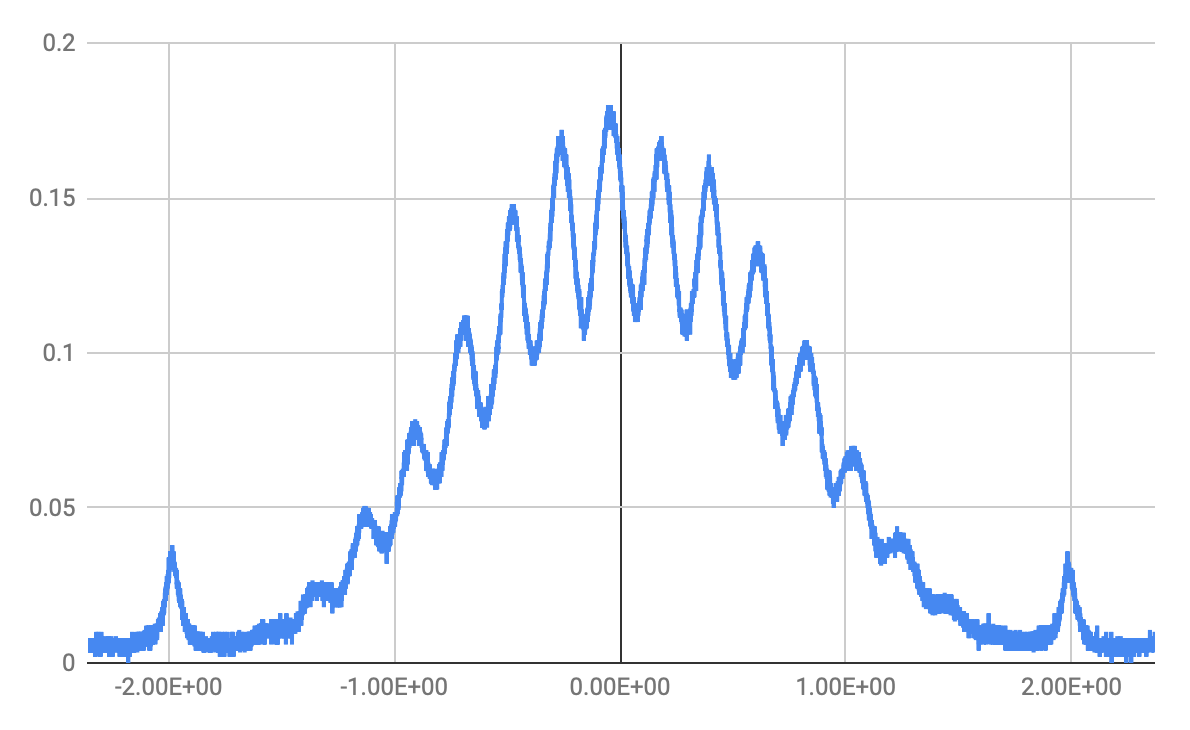
\includegraphics[width=0.4\linewidth]{2_7_spread_2GHz.png}}
    ~~~~
    \subcaptionbox
        {週期 $2^{7}-1$ 位元之偽隨機訊號
        \label{fig:subfig_fig2}}
        {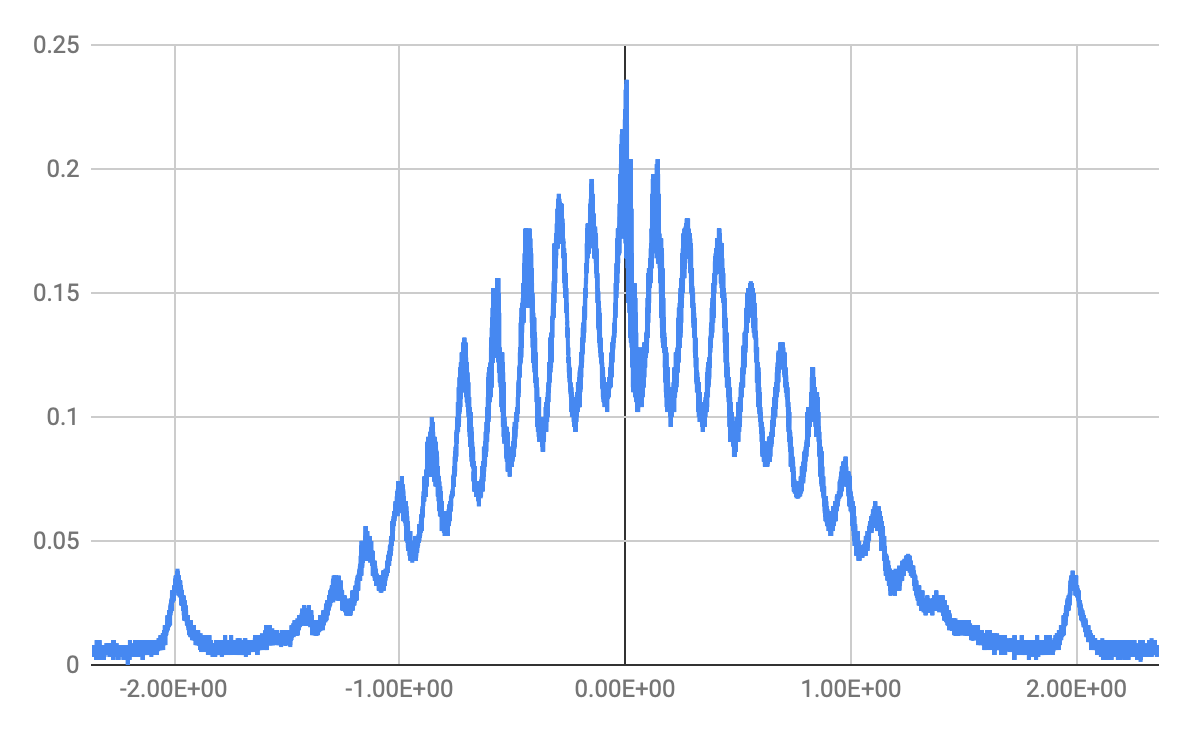
\includegraphics[width=0.4\linewidth]{2_15_spread_2GHz.png}}
    \caption{偽隨機訊號週期與展頻頻譜震盪之關係}
    \label{fig:different_length_PRBS}
\end{figure}

從以上測量的頻譜可以看出,調製後的頻寬與理論計算的結果一致,所以我們認為 10 Gb/s 的隨機訊號能將訊號展至 $\pm$10 GHz 寬。

\subsection{10 Gb/s 隨機訊號之相位調製}

當兩台 EOM 同時開啟時,理論上要能將展寬的頻譜還原成調製前的狀態,但從\cref{fig:10gbs_compress_sprectrum} 的實驗結果可以看出,壓縮回來的頻譜與調製前相比,中心頻率的強度僅為本來的 80\%,若將電壓放大來看(如\cref{fig:compress_amplified_compare})可以觀察到,在調製前所有能量皆集中於中心頻率附近,但經過兩台 EOM 調製後,仍有部分能量分散在其他頻率沒被還原,導致中心頻率的強度降低。造成頻譜還原效果不佳的可能原因為,兩個隨機訊號的形狀與穩定度皆不同(如\cref{fig:amplified_signal}),使相位無法被反向調製,還原成最初的狀態。

\fig[0.75][fig:10gbs_compress_sprectrum][!htb]{compress_comparison_100.png}[10 Gb/s 訊號壓縮後頻譜]

\fig[0.75][fig:compress_amplified_compare][!htb]{compress_zoom_in.png}[放大後之電訊號,紅線為未經調製的雷射頻譜,黑線為兩次調製後的訊號,雖能大致上將頻寬從 10 GHz 壓回 60 MHz,但從圖中可發現,中心以外的頻率仍能測到一些訊號。][初始頻譜與壓縮頻譜放大比較圖]

\begin{figure}[!hbt]
    %\captionsetup[subfigure]{labelformat=empty} % 完全隱藏圖號
    \centering
    \subcaptionbox
        {第一台 EOM 
        \label{fig:subfig_fig1}}
        {\includegraphics[width=0.4\linewidth]{amp_data.bmp}}
    ~~~~
    \subcaptionbox
        {第二台 EOM
        \label{fig:subfig_fig2}}
        {\includegraphics[width=0.4\linewidth]{amp_data_bar.bmp}}
    \caption{經過放大器,進入 EOM 用以調製的兩組隨機訊號眼圖}
    \label{fig:amplified_signal}
\end{figure}

\section{經相位調製後之 $^{87}Rb$ 原子吸收譜}

如\cref{section:simulation_absorption} 所提,當光子的頻率很接近原子的躍遷能階時,光會被吸收,實驗上可以\cref{fig:laser_spectrum_setup}的架設,將 Farby-Perot 干涉儀換成光二極體 (photodiode) 收光,連續調變入射光的頻率,測量透射 $^{87}Rb$ 原子氣體管的光強,從\cref{fig:abs_spec} 藍線可以觀察到,在特定的兩個頻率位置附近光會被原子吸收,穿透率特別低。本實驗主要的目的為透過展頻技術,降低光子與原子的交互作用,使光子能不被吸收而增加透射率,所以若將第一台 EOM 開啟,將雷射的頻寬從 60 MHz 展至 10 GHz,此時的吸收譜如\cref{fig:abs_spec} 紅線,在經過展頻後,無論在哪個頻率下光皆能大部分透射原子,調製前的光在 105 GHz 與 112 GHz 會被完全吸收,調製後卻有 75\% 的光能透射原子,就如隱形了一般,展頻能降低光子受環境的影響。

\fig[0.75][fig:abs_spec][!htb]{absorption_spectrum_spread.png}[調製後的如原子吸收譜,黑線為沒放 $^{87}Rb$ 原子氣體管時的訊號;藍線為調製前 $^{87}Rb$ 原子氣體管的吸收譜;紅線為展頻後的吸收譜。][調製後的銣原子吸收譜]

\section{單光子相位調製對原子吸收之影響}
從前一小節的實驗結果能得知,$^{87}Rb$ 的躍遷頻率約在 105 GHz 與 112 GHz 附近,這時我們將光源從窄頻雷射換成單光子,並透過改變入射光的頻率與晶體溫度,將單光子的頻率調至 112300 MHz,使其能被原子吸收,再以\cref{fig:single_photon_no_etalon} 的光路架設對光子進行相位調製與測量。

\fig[0.75][fig:single_photon_no_etalon][!htb]{single_photon_no_etalon_setup.png}[單光子量測光路圖]

當兩台 EOM 皆關閉時,頻寬約為 4.5 MHz 的單光子會幾乎完全被原子吸收,光無法透射氣體管,但若對其進行 $G^{2}(\tau)$ 測量,卻會測到訊號,如\cref{fig:remaining_mod_g2},原因如\cref{subsection:single_photon} 所述,是由於我們晶體產生的單光子源非單模 (single-mode),其中還存在符合其他組準相位匹配條件 (quasi phase matching condition) 所產生的光,若要去除那些光子對實驗的影響,在此小節的數據處理上,我們直接將其當作雜訊扣除,只保留主要模態的光;下一小節的實驗中,我們會外加一個 Etalon 濾波器,只讓 112300 MHz 附近的光通過。

\fig[0.75][fig:remaining_mod_g2][!htb]{initial_heatcell_no_etalon.png}[單光子通過 $^{87}Rb$ 原子氣體管之 $G^{2}(\tau)$ 量測,黑線為沒放氣體管時測到的訊號,放了氣體管後,其他模態的光因不在吸收頻率附近而能透射原子團不吸收,所以會測到紅線的訊號。][單光子通過 $^{87}Rb$ 原子氣體管之 $G^{2}(\tau)$ 量測]

若開啟第一台 EOM,以 10 Gb/s 的隨機訊號對單光子進行相位調製,可以讓單光子的頻寬從 4.5 MHz 展至 10 GHz,使大部分的光可以透射 $^{87}Rb$ 原子氣體不被吸收,扣除雜訊後的 $G^2(\tau)$ 的測量結果如\cref{fig:spread_absorption_g2},本該被原子吸收的光,因展頻而有 76\% 的透射率。

此時若將第二台 EOM 也開啟,使頻譜被壓縮且還原,再進行 $G^2(\tau)$ 測量,結果如\cref{fig:compress_absorption_g2},與\cref{fig:spread_absorption_g2} 相比,兩者單位時間測得的光子數幾乎相同,可知相位調製僅會改變頻率的分佈,不會影響光強。


\begin{figure}[!hbt]
    %\captionsetup[subfigure]{labelformat=empty} % 完全隱藏圖號
    \centering
    % \subcaptionbox
    %     {沒放 $^{87}Rb$ 原子氣體管
    %     \label{fig:no_cell_no_etalon}}
    %     {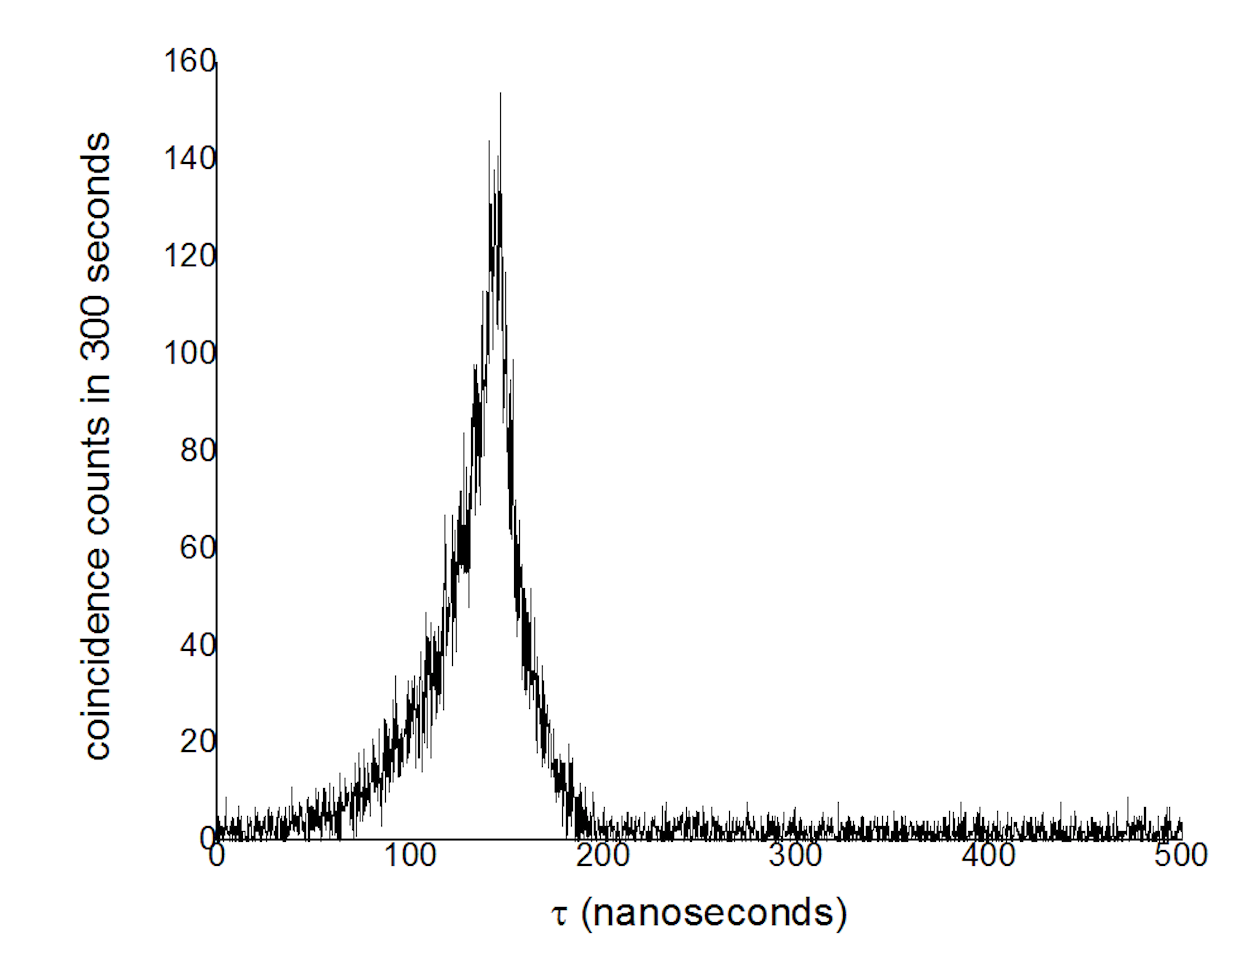
\includegraphics[width=0.3\linewidth]{nocell_no_etalon.png}}
    % ~~~~
    \subcaptionbox
        {只開第一台 EOM
        \label{fig:spread_absorption_g2}}
        {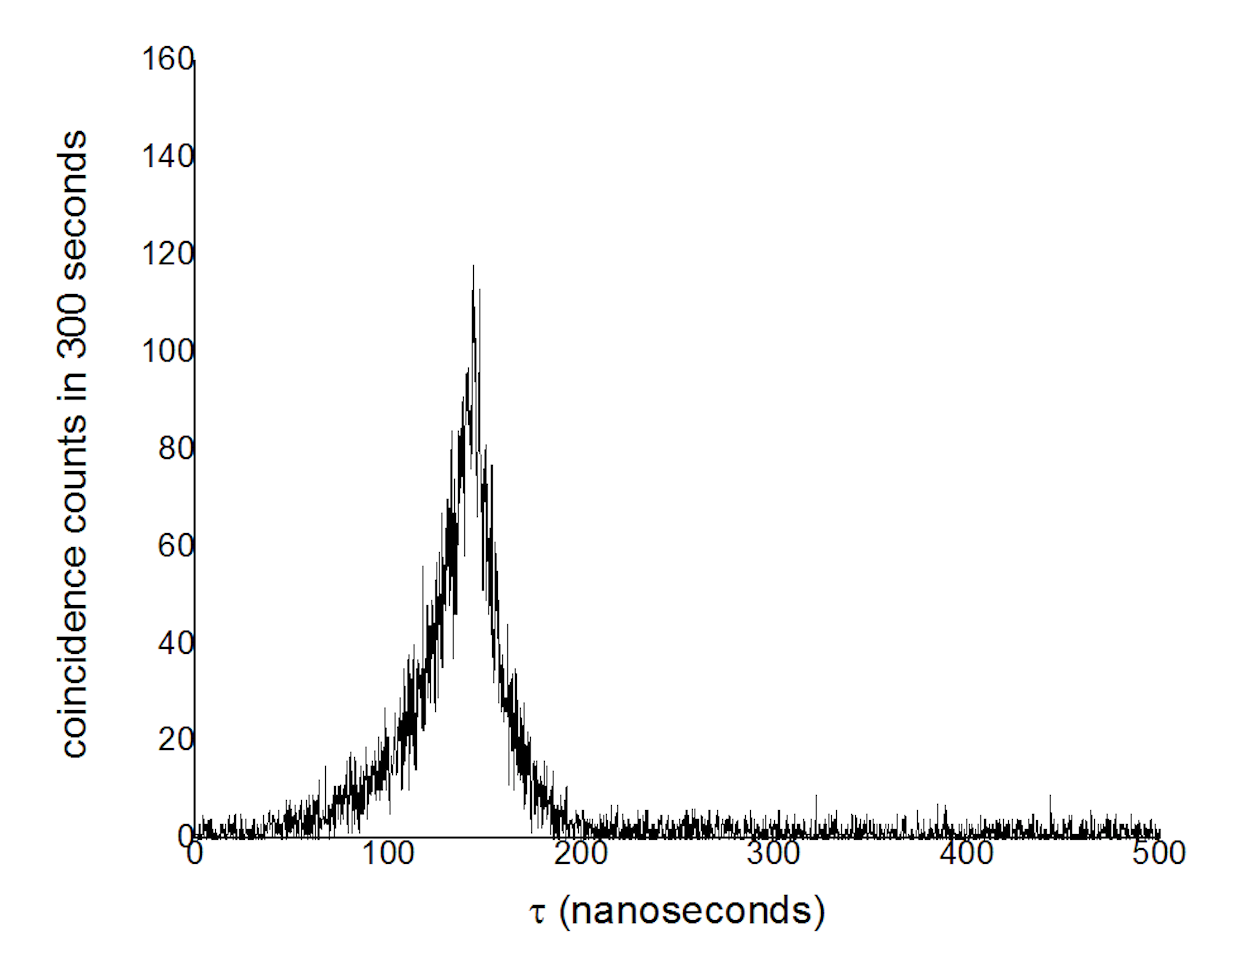
\includegraphics[width=0.4\linewidth]{heatcell_spread_no_etalon.png}}
    ~~~~
    \subcaptionbox
        {同時開啟兩台 EOM
        \label{fig:compress_absorption_g2}}
        {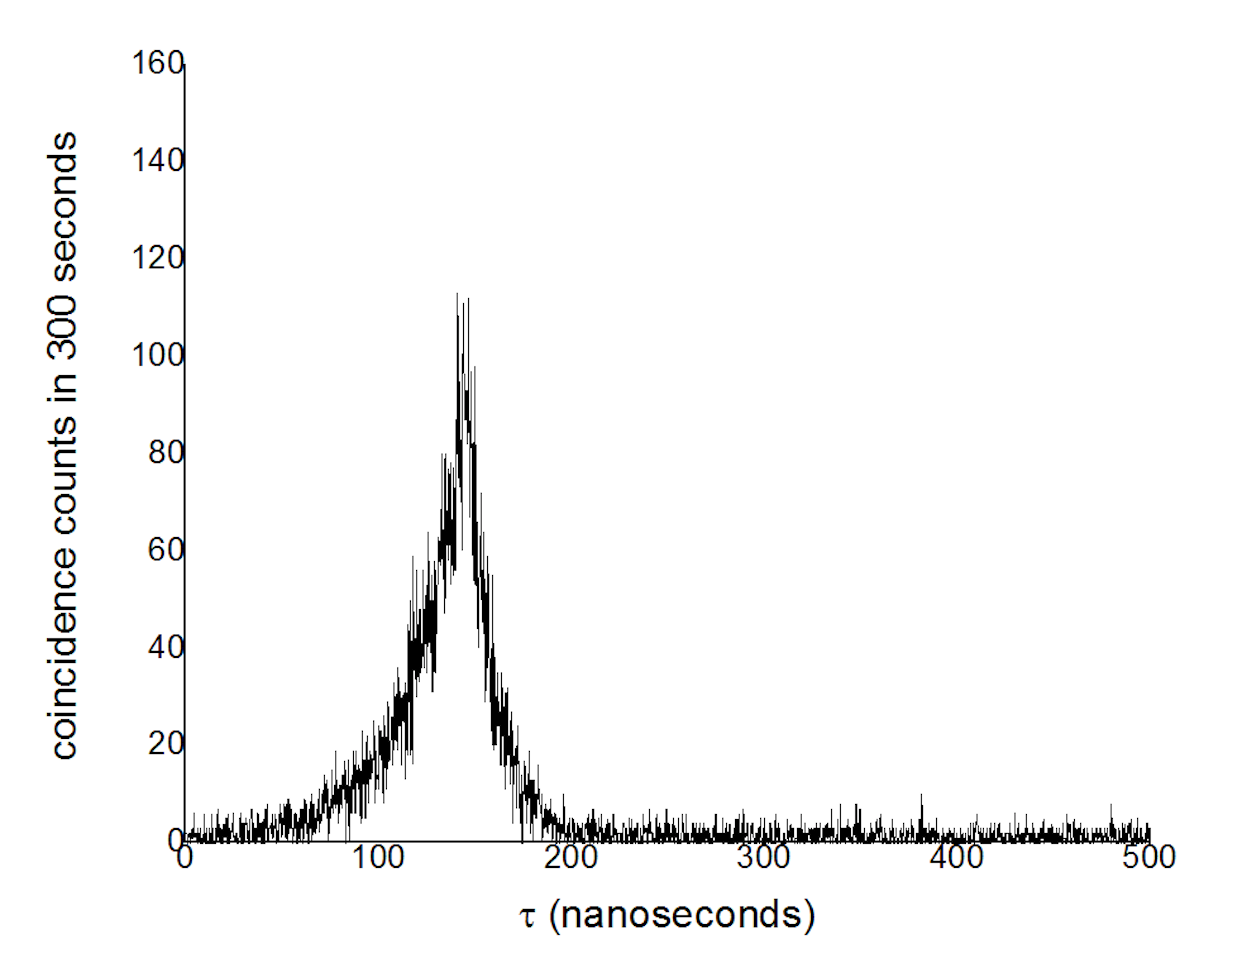
\includegraphics[width=0.4\linewidth]{heatcell_compress_no_etalon.png}}
    \caption{相位調製不影響波形與光強,僅改變頻率的分佈。}
    \label{fig:spread_or_not}
\end{figure}

從前述的結果可知,未經調製的窄頻單光子會幾乎被 $^{87}Rb$ 原子吸收,無法透射氣體管,透射率幾乎為零,但經過 10 Gb/s 隨機訊號的調製後,可讓透射率提升至 76%,如同穿上隱形斗篷般,能大部分的光子不會與原子產生交互作用,直接穿透原子團。

\section{雷射光相位調製對原子吸收之影響}
在上一小節中,我們對單光子進行相位調製,觀察展頻對吸收率之影響,為確定此現象在不同系統下能維持一致性,我們將\cref{fig:single_photon_no_etalon}光路架設的光源改為雷射光,單光子探測器改用光二極體,並將雷射調至與單光子同樣的波長去進行相同的量測,實驗結果如\cref{fig:laser_no_etalon},與單光子的量測結果相近,調製前的光幾乎會全部被原子團吸收,但經過展頻後的雷射光能有約 80\% 的穿透率,也能達到隱形斗篷的效果。

\fig[0.75][fig:laser_no_etalon][!htb]{laser_no_etalon.png}[雷射光相位調製對穿透率之影響,最上面三條線(藍、紅與黃色)為沒放$^{87}RB$ 原子氣體管時之量測,無論是展頻還是壓縮,相位調製皆不會影響光強;中間兩條線(綠色與橘色)為展頻後通過氣體管所測得的訊號,約 80\% 的光能因相位調製而穿透原子團而不被吸收;最下面的藍線為兩台 EOM 關閉時測到的訊號,未經調製的光會幾乎都被原子吸收。][雷射光相位調製對穿透率之影響]

\section{不同展頻頻寬對吸收率之影響}
由\cref{section:simulation_absorption} 的模擬可知,使用越高頻的隨機訊號去展頻可提升光子隱形的效果,為驗證此理論,我們分別使用 2, 4, 6, 8, 10 Gb/s 的隨機訊號去展頻,並透射原子團測量穿透率,實驗結果如\cref{fig:different_gbs_abs},從結果可看出,無論是雷射光或單光子,頻寬越大,吸收率越低,使用越高的頻率去進行調製,的確能增加光子的隱匿性,降低環境或竊聽者的影響。

\fig[0.75][fig:different_gbs_abs][!htb]{main_result.png}[黑色為數值模擬;紅線與藍線分別為雷射光與單光子的實驗測量結果,數據點的值為數次測量的平均,帶狀的寬度為測量的標準差。單光子的實驗結果標準差較大是由於晶體溫控穩定度不夠造成的。][改變展頻頻率對吸收率之影響]

此外,可以看出單光子的透射率皆比雷射光低一些,或許是因為單光子較容易被原子團吸收所致。

\section{單光子頻譜壓縮}

從前兩小節的結果可知,使用展頻技術可以有效的降低環境對光子的影響,但若考量到接收訊息端可能會需要光子原始的相位資訊,或者需要讓光子與 $^{87}Rb$ 原子進行交互作用,我們必須要開啟第二台 EOM 進行反向的調製,盡量使光子還原到原先的狀態,若以\cref{fig:single_photon_no_etalon} 的光路架設,除了第一台 EOM 外,將第二台也開啟,由於相位調製不影響光強與波形,單就 $G^{2}(\tau)$ 的測量無法得知頻譜的變化,因此要將光路架設改為\cref{fig:single_photon_with_etalon},在單光子探測器前加上 Etalon 濾波器,限制只讓頻寬 60 MHz 內的光通過,如此一來,只要能測到訊號就代表部分光子的頻寬有被壓窄至 60 MHz 內,另一方面,這也可以將上一小節及提的雜訊去除。

\fig[0.75][fig:single_photon_with_etalon][!htb]{single_photon_with_etalon_setup.png}[加上濾波器之單光子量測光路圖]

以\cref{fig:single_photon_with_etalon} 的光路架設,只開啟第一台 EOM 時,被展頻的單光子能大部分透射原子團,但由於 Etalon 的過濾,頻寬 10 GHz 的光子幾乎無法抵達探測器,因而測不到明顯的訊號,結果如\cref{fig:spread_single_photon_with_etalon}。若將第二台 EOM 也開啟,將已展頻且被部分吸收的單光子頻譜壓縮,則能再次測到訊號,如\cref{fig:compress_single_photon_with_etalon},與調製前且沒放氣體管時的初始訊號相比,透射率為 42.3\%。

\begin{figure}[!hbt]
    %\captionsetup[subfigure]{labelformat=empty} % 完全隱藏圖號
    \centering
    \subcaptionbox
        {只開啟第一台 EOM,將展頻單光子通過原子團,雖然能大部分透射不被吸收,但由於光子的頻寬 10 GHz,遠小於 Etalon 濾波器的 60 MHz,所以測不到訊號。
        \label{fig:spread_single_photon_with_etalon}}
        {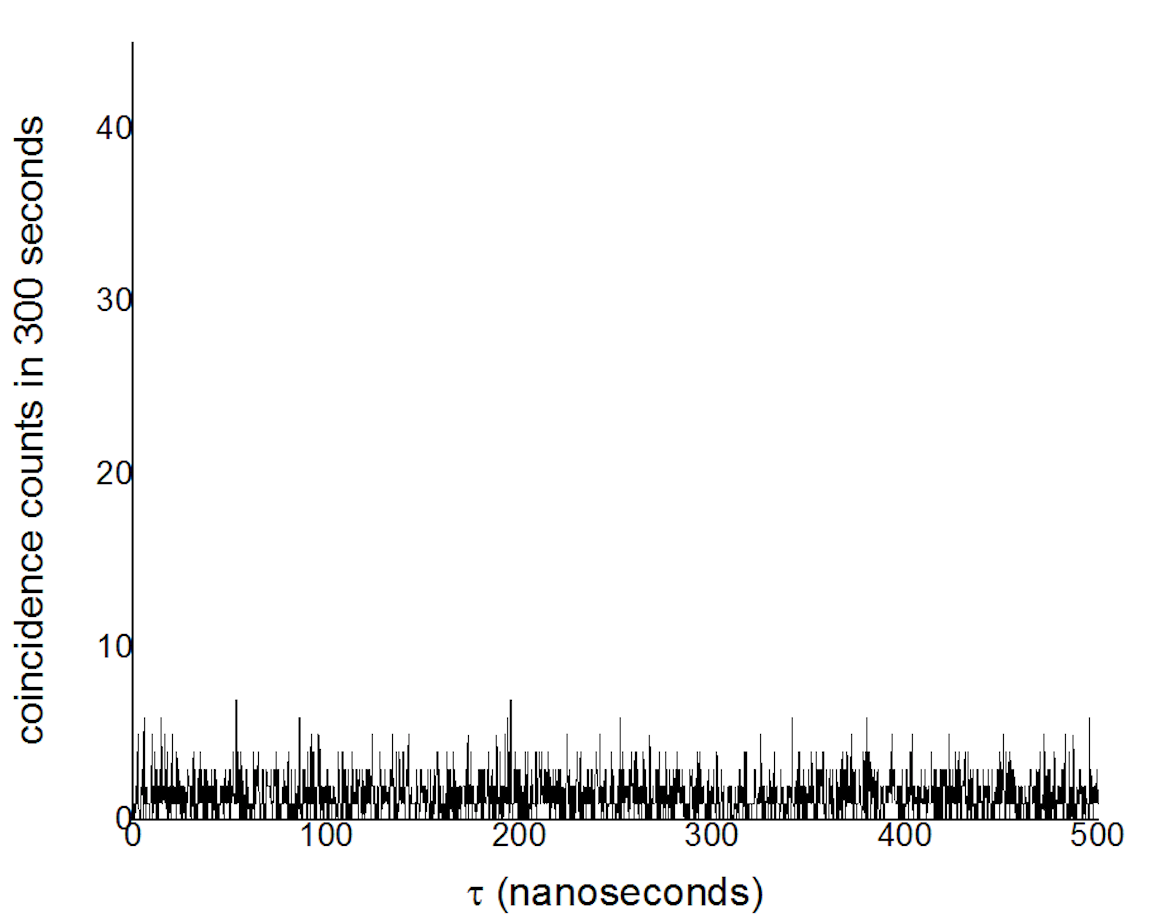
\includegraphics[width=0.4\linewidth]{heat_cell_spread_with_etalon.png}}
    ~~~~
    \subcaptionbox
        {兩台 EOM 同時開啟,將已展頻的單光子頻譜壓縮,使光子再次現形,能透射 Etalon 濾波器,被探測器偵測到。
        \label{fig:compress_single_photon_with_etalon}}
        {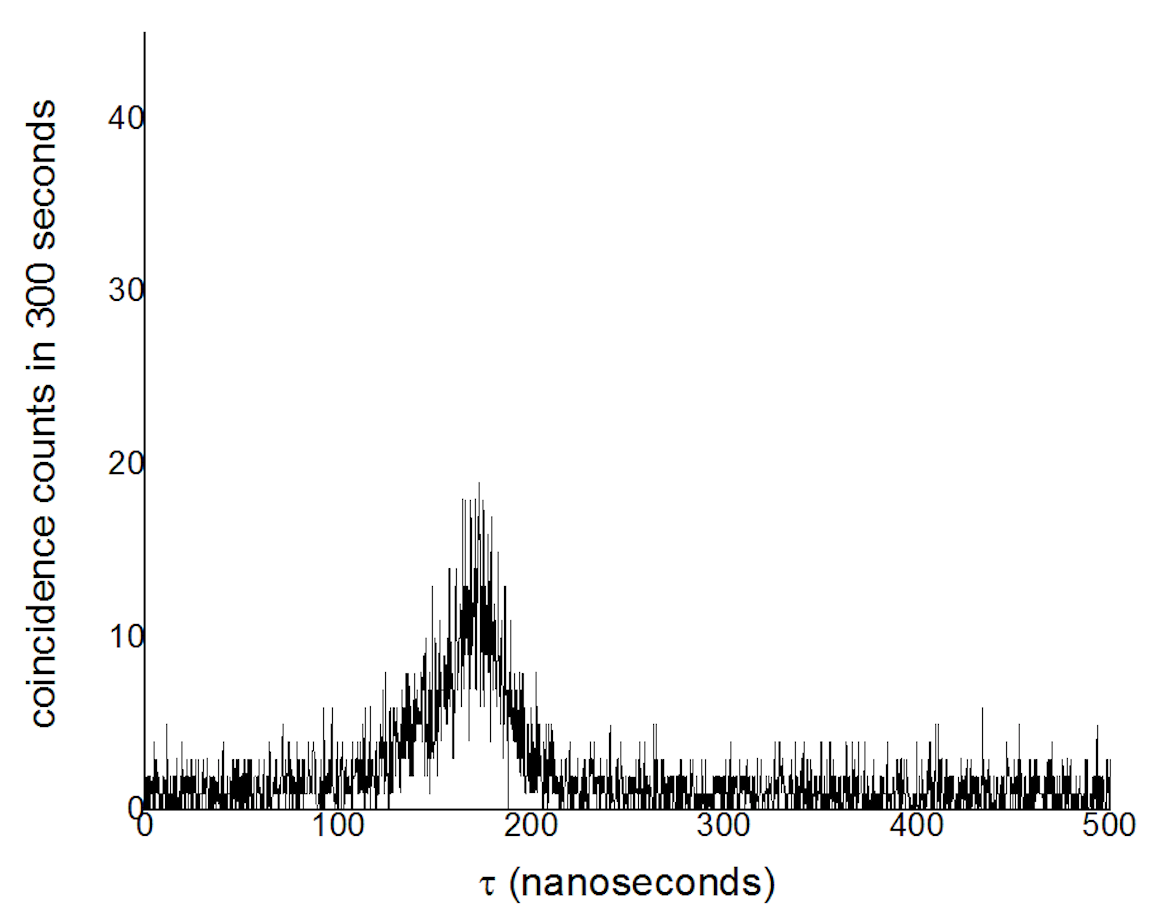
\includegraphics[width=0.4\linewidth]{heat_cell_compress_with_etalon.png}}
    \caption{加上 Etalon 濾波器之單光子 $G^{2}(\tau)$ 量測}
    \label{fig:single_photon_with_etalon}
\end{figure}

為了知道原子吸收對於單光子頻譜的壓縮有何影響,我們以同樣的光路架設,在沒放 $^{87}Rb$ 原子氣體管時同時開啟兩台 EOM,測量結果如\cref{fig:compress_compare_with_etalon}黑線,與調製前的訊號相比,透射率為 77.9\%;放上 $^{87}Rb$ 原子氣體管後的訊號為紅線,透射率為 42.3\%。

\fig[0.75][fig:compress_compare_with_etalon][!htb]{compress_compare_with_etalon.png}[在兩台 EOM 同時開啟時測量 $G^{2}(\tau)$,黑線為沒經過 $^{87}Rb$ 原子氣體管時之量測;紅線為透射 $^{87}Rb$ 原子氣體管之訊號,兩者的比值為 54.3\%。][原子吸收對單光子壓縮比較圖]

\section{雷射光頻譜壓縮}

同樣的,我們以上一小節相同的架設,將光源換成雷射光,單光子探測器改為光二極體,且進行同樣的測量,結果如\cref{fig:no_cell_compress_laser},與單光子的量測結果相近,經展頻後再壓縮的光,約 70\% 能通過 Etalon 濾波器,若在中間放氣體管使部分光被吸收,僅 40\% 的光能通過 Etalon,被重新壓回窄頻雷射

\fig[0.75][fig:no_cell_compress_laser][!htb]{laser_modulation_with_etalon.png}[原子吸收對雷射光壓縮品質比較圖]

\section{誤差分析與模擬修正}

由相位調製的基本原理可知,若輸入兩台 EOM 的隨機訊號符合\cref{eq:prbs_condition} 的條件,則能完美的將光的相位與頻譜還原成最初的狀態,在我們實驗中所使用的窄頻雷射與單光子,頻寬皆遠小於 Etalon 濾波器的頻寬,在沒原子團吸收的狀況下,被展頻再壓縮的光應該要能 100\% 通過 Etalon,這與實驗測量的結果不符,我認為主要的可能原因為隨機訊號的品質不佳所致,兩個訊號從 PRBS 輸出時的波形如\cref{fig:prbs_eye_},兩者形狀不一致,且上下不對稱,若在經過延長線與高頻訊號放大器波形則變為\cref{fig:amp_prbs_eye},兩者變得更不一致,有著不一樣的波形、穩定度、上升時間、下降時間與交叉位置 (crossing),這些因素都會使兩台 EOM 的調製無法互相抵消,讓相位無法還原至最初的狀態。除此之外,也有能是因為兩台 EOM 對高頻訊號的響應不同,也會影響調製的結果。

\begin{figure}[!hbt]
    %\captionsetup[subfigure]{labelformat=empty} % 完全隱藏圖號
    \centering
    \subcaptionbox
        {第一台 EOM
        \label{fig:subfig_fig1}}
        {\includegraphics[width=0.4\linewidth]{data.bmp}}
    ~~~~
    \subcaptionbox
        {第二台 EOM
        \label{fig:subfig_fig2}}
        {\includegraphics[width=0.4\linewidth]{data_bar.bmp}}
    \caption{PRBS 輸出之訊號眼圖(放大前)}
    \label{fig:prbs_eye_}
\end{figure}

\begin{figure}[!hbt]
    %\captionsetup[subfigure]{labelformat=empty} % 完全隱藏圖號
    \centering
    \subcaptionbox
        {第一台 EOM
        \label{fig:subfig_fig1}}
        {\includegraphics[width=0.4\linewidth]{amp_data.bmp}}
    ~~~~
    \subcaptionbox
        {第二台 EOM
        \label{fig:subfig_fig2}}
        {\includegraphics[width=0.4\linewidth]{amp_data_bar.bmp}}
    \caption{PRBS 輸出之訊號眼圖(放大後)}
    \label{fig:amp_prbs_eye}
\end{figure}

為了確認上述的因素所造成的影響,根據\cref{fig:amp_prbs_eye}的測量結果,修正模擬時使用的隨機訊號,修正的參數如\cref{tab:paras},模擬的電訊號如\cref{fig:modify_or_not}。

\begin{figure}[!hbt]
    %\captionsetup[subfigure]{labelformat=empty} % 完全隱藏圖號
    \centering
    \subcaptionbox
        {修正前
        \label{fig:subfig_fig1}}
        {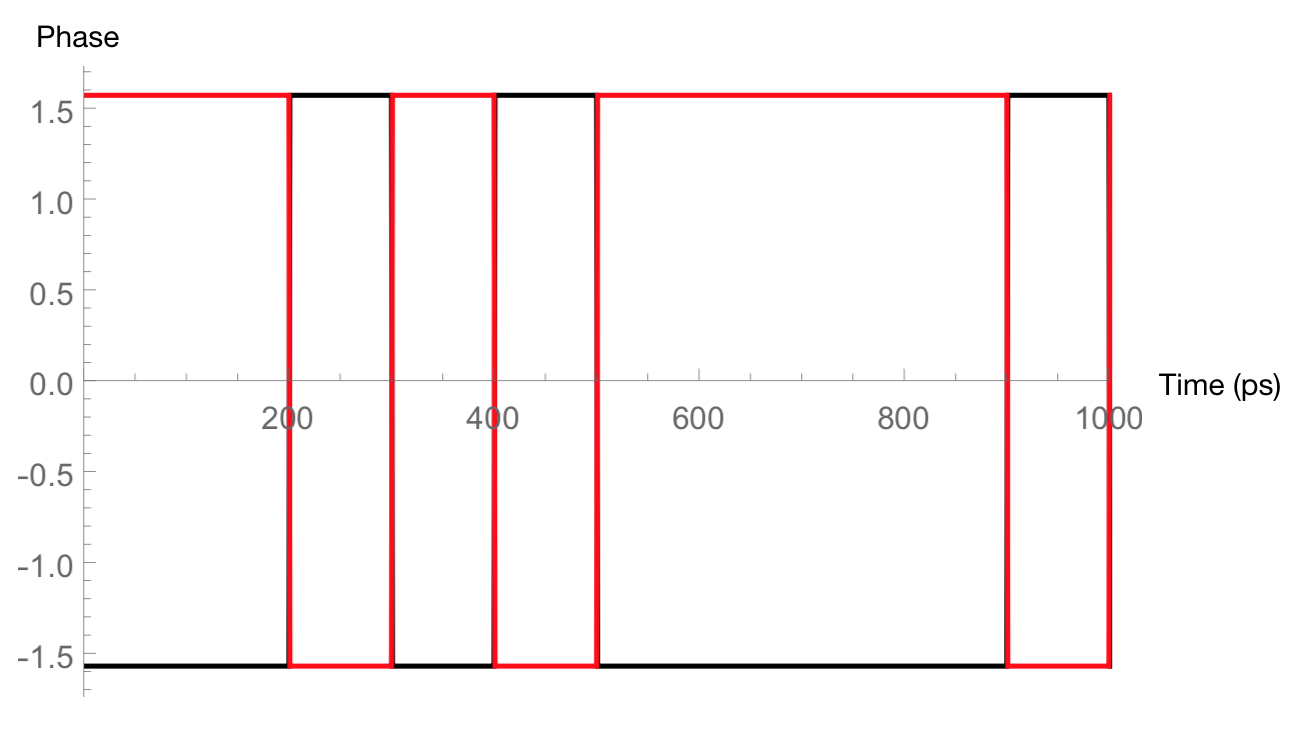
\includegraphics[width=0.4\linewidth]{10gbs_prbs.png}}
    ~~~~
    \subcaptionbox
        {修正後
        \label{fig:subfig_fig2}}
        {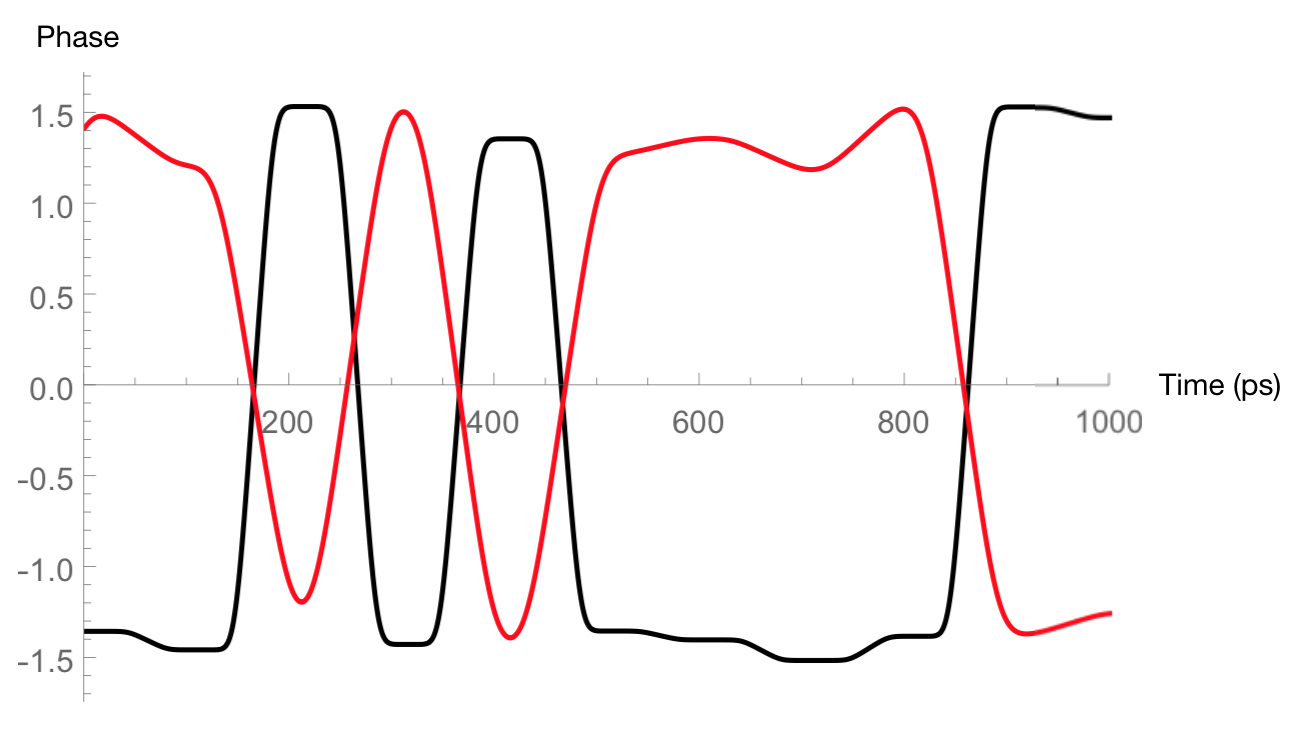
\includegraphics[width=0.4\linewidth]{10gbs_prbs_rf.png}}
    \caption{理論模擬使用的隨機訊號,黑線與紅線分別為輸入第一台和第二台 EOM 之電訊號。}
    \label{fig:modify_or_not}
\end{figure}

使用修正後的隨機訊號進行展頻、吸收與壓縮的模擬,可讓計算的結果更貼近實驗的測量,以下將整理理論與實驗的結果整理成\cref{tab:spread_abs} 與\cref{tab:compress_abs},從表中可觀察到,經過修正後的理論模擬更接近實驗的結果,由此可知,想要有效地使用展頻技術,電訊號的品質起了關鍵的作用,需要有更好的訊號產生器與線材才可以將調製的訊號還原成原始的模樣。

\begin{table}[h]
    \centering
    \caption{數值模擬參數修正}
    \begin{tabular}{| c | c | c | c |}
\hline
         & jitter & amplitidu & rising \& falling
    \\ \hline
    \ce{EOM 1} & 14 ps & $\pm$7.7\% & 38 ps\\ \hline
    \ce{EOM 2} & 16 ps & $\pm$16.7\% & 144 ps\\ \hline
    \end{tabular}
    \label{tab:paras}
\end{table}

\begin{table}[h]
    \centering
    \caption{展頻後的光經過 $^{87}Rb$ 原子氣體管之透射率(無 Etalon 濾波器)}
    \begin{tabular}{| c | c | c | c | c |}
\hline
\multirow{2}{*}{無 Etalon}& \multicolumn{2}{c|}{ 理論 } & \multicolumn{2}{c|}{ 實驗 }
\\ \cline{2-5}
         & 修正前 & 修正後 & 雷射光 & 單光子
    \\ \hline
    穿透率 & 79.1\% & 73.8\% & 77.38\% & 68.48\%\\ \hline
    \end{tabular}
    \label{tab:spread_abs}
\end{table}

\begin{table}[h]
    \centering
    \caption{展頻後壓縮的光經過 Etalon 濾波器之透射率}
    \begin{tabular}{| c | c | c | c | c |}
\hline
    \multirow{2}{*}{有 Etalon}& \multicolumn{2}{c|}{ 理論 } & \multicolumn{2}{c|}{ 實驗 }
    \\ \cline{2-5}
        & 修正前 & 修正後 & 雷射光 & 單光子
    \\ \hline
    無通過氣體管 & 100.0\% & 88.9\% & 77.9\% & 70.9\%\\ \hline
    有通過氣體管 & 67.6\% & 45.6\% & 42.3\% & 41.0\%\\ \hline
    \end{tabular}
    \label{tab:compress_abs}
\end{table}

\todo[inline]{補上模擬圖}
\end{document}          % 實驗結果與討論
        \documentclass[class=NCU_thesis, crop=false]{standalone}
\begin{document}

\chapter{總結}
展頻好棒棒
是一個想起來很簡單,做起來很靠腰的一個實驗

\end{document}      % 結論
%        \documentclass[class=NCU_thesis, crop=false]{standalone}
\usepackage{showexpl}

\begin{document}

\chapter{章名(章節示例)}
章內容內容內容內容內容 \\
內容內容內容

\section{節名}
節內容內容內容內容內容 \\
內容內容內容

\subsection{小節名}
內容內容內容 \\
內容內容內容

\subsubsection{小小節}
內容內容內容 \\
內容內容內容

\paragraph{段}
內容內容內容 \\
內容內容內容

\subparagraph{小段}
內容內容內容 \\
內容內容內容


\chapter{文字}
第一行。
仍是第一行。 \\
第二行。


\chapter{圖片}
\section{插入單一圖片}
\fig[0.15][fig:label_test][!hbt]{logo-Linux.png}[caption][short caption]

\section{插入多張圖片}
\begin{figure}[!hbt]
    %\captionsetup[subfigure]{labelformat=empty} % 完全隱藏圖號
    \centering
    \subcaptionbox
        {caption\_1
        \label{fig:subfig_fig1}}
        {
\includegraphics[width=0.3\linewidth]{fig1.png}}
    ~
    \subcaptionbox
        {caption\_2
        \label{fig:subfig_fig2}}
        {
\includegraphics[width=0.3\linewidth]{fig2.eps}}
    \vspace{\baselineskip} % 分隔上下列
    \subcaptionbox
        {caption\_3
        \label{fig:subfig_fig3}}
        {
\includegraphics[width=0.6\linewidth]{fig3.png}}
    \caption{caption, 使用 \subref{fig:subfig_fig2}取得子圖(Debian)編號 }
    \label{fig:label}
\end{figure}


\chapter{表格}
\section{一般表格}
\begin{table}[h]
    \centering
    \caption{Solution}
    \begin{tabular}{| l | l |}
        \hline
        Component & Concentration(mM) \\ \hline
        \ce{NaCl} & 118.0 \\ \hline
    \end{tabular}
\end{table}

\section{自動折行表格}
\begin{table}[h]
    \centering
    \begin{tabularx}{\textwidth}{| l | X |}
        \hline
        short & short short \\ \hline
        long & long long long long long long long long long long  long long long long long long long long long long\\ \hline
    \end{tabularx}
\end{table}

\end{document}
    \backmatter          % book class 預設\backmatter 在\appendix 後面。因此.cls修改過\appendix 定義
        % This file has 3 types bibliography management, 
% \bibManType in config.tex choose it.
% 0. Embedded: write \bibitem in {thebibliography} environment.
% 1. BibTeX: Change bib files in \bibliography{}
% 2. biber / BibLaTeX: Add bibliography by \addbibresource{bibfile.bib} in macros_preamble.tex

\documentclass[class=NCU_thesis, crop=false]{standalone}

\begin{document}

\ifcase \bibManType 
    % 0 == Embedded %%%%%%%%%%%%%%%%%%%%%%%%%%%%%%%%%%%%%%%
    {\bibFontStyle\setstretch{\bibLineStretch}
    \begin{thebibliography}{99}

    \bibitem{cite_key_1}
        bibliography item detail.

    \bibitem{_sppmg/tw_thesis_template_????}
        TW\_Thesis\_Template,
        sppmg,
        \url{https://github.com/sppmg/TW_Thesis_Template},
        Embedded bibliography demo.

    \end{thebibliography}
    }
    
\or
    % 1 == BibTeX %%%%%%%%%%%%%%%%%%%%%%%%%%%%%%%%%%%%%%%%%
    \bibliographystyle{\bibStyle}
    {\bibFontStyle\setstretch{\bibLineStretch}
        \bibliography{demo} % {sample_1,sample_2,...,sample_n}
        % Note the lack of whitespace between the commas and the next bib file.
    }
\or

    % 2 == biber / BibLaTeX %%%%%%%%%%%%%%%%%%%%%%%%%%%%%%%
    \printbibliography[title = {參考文獻}, heading = bibnumbered]
\fi



\end{document}
    \appendix
%         \documentclass[class=NCU_thesis, crop=false]{standalone}
\begin{document}

\definecolor{Gray3}{gray}{0.8}

\chapter{Solutions}

\section{The solution}
\begin{table}[!h]
    \centering
    \begin{tabular}{| l | l |}
        \hline
        Component & Concentration(mM) \\ \hline
        \rowcolor{Gray3}
        \ce{NaCl} & 1.0 \\ \hline
        \ce{CaCl_2} & 2.0 \\ \hline
        \rowcolor{Gray3}
        \ce{NaCl} & 1.0 \\ \hline
        \ce{CaCl_2} & 2.0 \\ \hline
    \end{tabular}
    \caption{The solution}
\end{table}
\end{document}
%         \documentclass[class=NCU_thesis, crop=false]{standalone}

\begin{document}
\chapter{自動填單}
這裡試著幫各位自動填入部份資訊,其餘打勾、日期請手寫。有字體大小不符、位置歪掉等問題的話,請修改 appendix\_letter\_NCU.tex後直接編譯生成文件。

appendix\_letter\_NCU.tex中,每個句子(文字項目)都是獨立的大小與位置。 大小可由\textbackslash{}fs,調整。
\footnote{\textbackslash{}fs 使用 \textbackslash{}fontsize 做無級調整,並固定單行高度。 }
位置可由\textbackslash{}placetextbox 調整。語法如下:
\begin{lstlisting}[style=LatexStyle,caption={}]
\placetextbox{x(mm)}{y(mm)}
\end{lstlisting}
單位使用mm ,(0,0)位於左下角。建議調整時將``colorgrid''加入documentclass選項。(加入子檔的即可)
\begin{lstlisting}[style=LatexStyle,caption={}]
\documentclass[class=NCU_thesis, crop=false, colorgrid]{standalone}
\end{lstlisting}
colorgrid 將顯示格線(一小格是\SI{5}{\milli\metre})。

\begin{center}
{ \noindent\color{red}\bfseries\Large NCU English letters in the NCU\_en}
\end{center}

%%%%%%%%%%%%%%%%%%%%%%%%%%%%%%%%

% define \mprof 
\ExplSyntaxOn
    % Copy prof. list from config.tex
    \clist_gclear_new:N \g_sppmg_profs_cl
    \clist_gset:NV \g_sppmg_profs_cl \profs
    \clist_gpop:NNTF \g_sppmg_profs_cl \l_tmpa_tl {}{ \tl_clear:N \l_tmpa_tl}
    \cs_gset_eq:NN \mprof \l_tmpa_tl
\ExplSyntaxOff

\cleardoublepage
\pagestyle{empty}
\sffamily
% ------------------------------

% % 碩博士論文電子檔授權書
\IfFileExists{\letterAuthEl}{
\cleardoublepage\thispagestyle{empty}
\includepdf[pagecommand={   \placetextbox{100}{120}{\fs{17}\title}%
                            \placetextbox{95}{109}{\fs{17}\mprof}%
                            \placetextbox{69}{98}{\fs{17}\deptshort} }]%
{\letterAuthEl}}{}

% 碩博士紙本論文延後公開/下架申請書。(如需延後公開者,才需要裝訂於論文內頁)
\IfFileExists{\letterPubReq}{
\cleardoublepage\thispagestyle{empty}
\includepdf[pagecommand={   \placetextbox{128}{270}{\fs{17}\author}%
                            \placetextbox{70}{258}{\fs{17}\deptshort}%
                            \placetextbox{100}{233}{\fs{17}\title}%
                            \placetextbox{90}{219.3}{\fs{17}\mprof} }]%
{\letterPubReq}}{}

% 指導教授推薦書
\IfFileExists{\letterRecom}{
\cleardoublepage\thispagestyle{empty}
\includepdf[pagecommand={   \placetextbox{50}{159}{\fs{22}\deptshort}%
                            \placetextbox{118}{159}{\fs{22}\author}%
                            \placetextbox{105}{144}{\fs{22}\title}}%
]{\letterRecom}}{}

% 口試委員審定書
\IfFileExists{\letterVerif}{
\cleardoublepage\thispagestyle{empty}
\includepdf[pagecommand={   \placetextbox{63}{200.5}{\fs{22}\deptshort}%
                            \placetextbox{145}{200.5}{\fs{22}\author}%
                            \placetextbox{100}{170}{\fs{22}\title}}%
]{\letterVerif}}{}

% ------------------------------
\pagestyle{fancy}
\end{document}
\end{document}
